\documentclass{article}
\usepackage[utf8]{inputenc}
\usepackage[T2A]{fontenc}
\usepackage[russian]{babel}
\usepackage{amsmath}
\usepackage{amssymb}
\usepackage{graphicx}
\usepackage{physics}

\begin{document}

\section*{Введение}
\textbf{Безынерционная цепь} --- это цепь, в которой отсутствует \textbf{запас энергии}. 
Это означает, что цепь реагирует на изменения мгновенно, без переходных процессов. Также 
это означает, что цепь не может накапливать заряд.
Для нас с вами это значит, что на этой лекции мы будем рассматривать цепи, состоящие только
 из резисторов и источников, и не будем иметь дело с конденсаторами и катушками. 

\section*{Топология цепи}
С точки зрения топологии цепь состоит из узлов и ветвей. \textbf{Узел} - это точка цепи, 
где соединяются три и более проводника. \textbf{Ветвь} - это участок цепи между двумя узлами.
Есть еще понятия двухполюсник, трехполюсник и так далее. \textbf{Двухполюсник} - это любой 
фрагмент электрической цепи, который имеет два вывода (``полюса'') для подключения к внешней 
схеме. По сути он представляет из себя черный ящик с торчащими наружу выводами. Трехполюсник
 тот же черный ящик, но уже с тремя выходами, и так далее. Ограничимся пока этими понятиями.

\section*{Методы расчета безынерционных цепей}
В школе вы уже сталкивались с задачами на расчет подобных цепей. Как правило для нахождения
неизвестных величин вы пользовались уравнениями Кирхгофа, а если еще проще то законом Ома.
 Сейчас же мы рассмотрим методы, которые позволяют систематизировать и упростить расчет цепей.

\subsection*{Законы Кирхгофа (напоминание)}
\textbf{Первый закон Кирхгофа} говорит о том, что алгебраическая сумма токов, втекающих в
 узел равна нулю. Проще говоря сумма втекающих в узел токов равна сумме вытекающих из узла токов.
$$
\sum_i I_i^{\text{in}} = \sum_j I_j^{\text{out}} 
$$
\textbf{Второй закон Кирхгофа} заключается в том, что алгебраическая сумма всех ЭДС и
 напряжений в любом замкнутом контуре равна нулю.
$$
\sum \limits_i IR_i = \sum\limits_j E_j
$$
\subsection*{Метод контурных токов}
Суть метода заключается в том, что мы разделяем цепь на набор замкнутых контуров и 
делаем замену исходных токов на \textbf{контурные токи}. Контурные токи на самом 
деле являются виртуальными, то есть воображаемыми, однако в силу того, что все уравнения,
 описывающие безынерционные цепи являются \textbf{линейными} (для них выполняется принцип суперпозиции),
мы можем произвести линейную замену одних токов на другие. Подробнее про линейность мы поговорим чуть позже.
Для лучшего понимания такой замены обратимся к простому примеру. Пусть по проводу течет ток в 3 ампера. 
Однако если мы представим этот ток как сумму двух токов в 5 ампер и 2 ампера, текущих в противоположных
 направлениях, суть происходящего не изменится.
$$
\begin{array}{l}
\qquad \qquad\text{3A}  \qquad \qquad \qquad  \qquad \qquad\text{5A} \\
---\longrightarrow--- \qquad \qquad ---\longrightarrow--- \\
\qquad \qquad \qquad \qquad \qquad \qquad \quad \qquad \text{2A} \\
\qquad \qquad \qquad \qquad \qquad \qquad --- \longleftarrow--- \\
\end{array}
$$
Разбивать цепь на контуры можно разными способами, однако проще всего делать это так, чтобы контуры
были как можно меньше и не содержали в себе других контуров.

Рассмотрим метод на примере несложной схемы. 
\begin{figure}[h!]
    \centering
    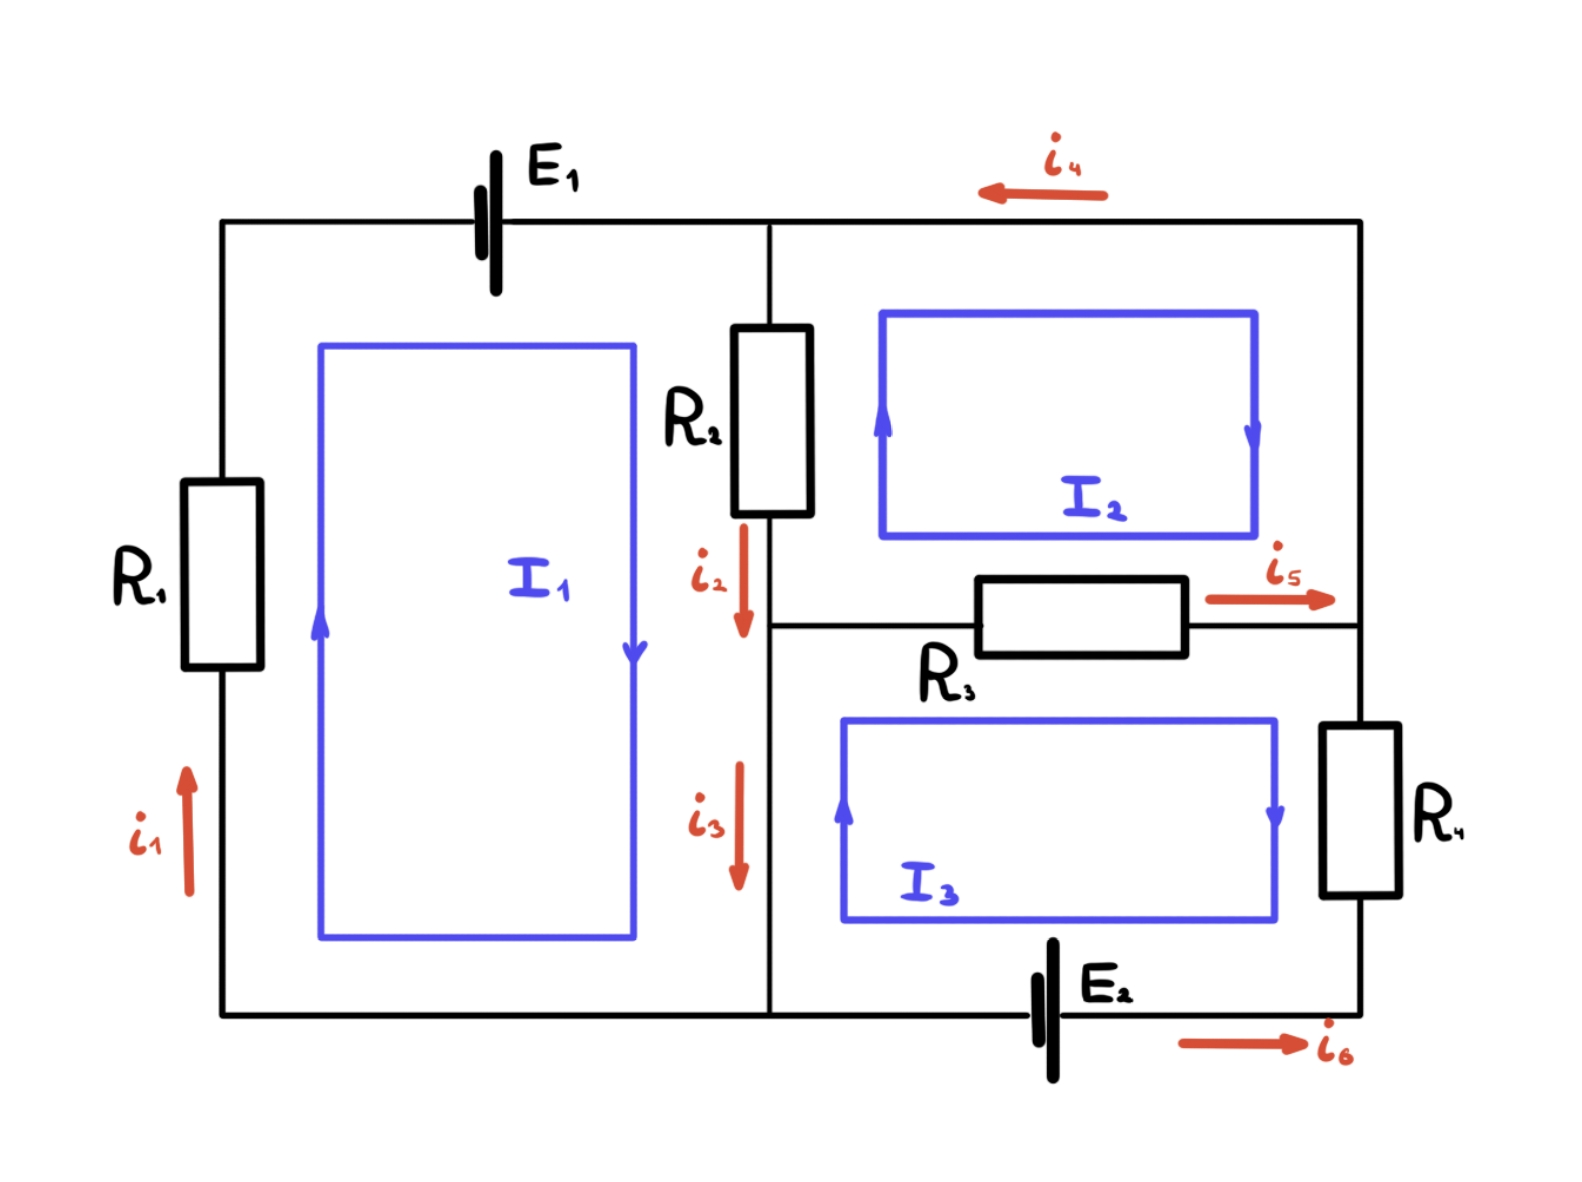
\includegraphics[width=0.9\textwidth]{Images/Metod_lonturnih_tokov.jpg}
    \caption{Схема для метода контурных токов}
    \label{fig:Metod_lonturnih_tokov}
\end{figure}
Выразим токи нашей схемы через контурные токи:
$$
\begin{matrix}
i_1 = I_1;          & i_4 = -I_2; \\
i_2 = I_1 - I_2;    & i_5 = I_3 - I_2; \\
i_3 = I_1 - I_3;    & i_6 = - I_3; \\
\end{matrix}
$$
Если мы найдем контурные токи, то сможем восстановить по ним и исходные токи.

Контурные токи мы будем искать, применяя второй закон Кирхгофа к каждому контуру.
Знаки перед слагаемыми зависят от направления обхода контура. Если ток течет вдоль направления 
обхода, то знак, с которым он входим в формулу - положительный. Если направление действия источника 
совпадает с течением тока, то в сумму он также входит со знаком плюс.
Для наших контуров это выражение выглядит так (направление обхода всегда по часовой):
$$\begin{array}{l}
I_1 (R_1 + R_2) - I_2 R_2 = E_1 \\
I_3 (R_2 + R_3) - I_1 R_2 - I_3R_3 = 0 \\
I_3 (R_3 + R_4) - I_2 R_3 = - E_2 \\
\end{array}$$
Таким образом мы получим систему линейных уравнений. Решив её, мы найдем контурные токи. Затем, 
совершив обратное преобразование, мы найдем исходные токи. 
\subsection*{Метод узловых потенциалов}
Этот метод существенно проще и многим знаком со школы. Он в каком-то смысле противоположен методу 
контурных токов, так как исследует узлы, а не ветви и использует первый закон Кирхгофа, а не второй. 
Напомню, что первый закон Кирхгофа говорит о том, что сумма втекающих в узел токов равна сумме вытекающих.
\begin{enumerate}
    \item Выберем один из узлов за ``землю'' - то есть присвоим ему потенциал равный нулю. Обозначим его $\varphi_0$.
    \item Остальные узлы цепи - это неизвестные величины, которые будут фигурировать в уравнениях. Обозначим их $\varphi_1, \varphi_2, \dots$
    \item Для каждого уравнения запишем первый закон Кирхгофа. Таким образом получим систему уравнения на токи.
    \item Каждый ток выразим через узловые потенциалы, в результате чего получим систему уравнений на узловые потенциалы.
    \item Зная потенциалы можно найти токи в каждой ветви.
\end{enumerate}

\section*{Двухполюсники}
Как уже было сказано, двухполюсник можно рассматривать как черный ящик, который имеет два выхода. 
С помощью этих выходов мы можем измерить силу протекающую через него тока $I$ и разность потенциалов 
на этих выходах $\Delta\varphi$, то есть напряжение $U$. Возникает вопрос, как эти две величины в двухполюснике связаны.
Рассмотрим двумерное векторное пространство ($I$, $U$). Какое множество в этих координатах может описывать 
двухполюсник? Скорее всего мы ожидаем увидеть кривую или даже график некоторой непрерывной функции. Почему 
именно непрерывной? Да потому что если бы график имел разрыв, то это означало бы, что при сколь угодно 
малом изменении одной переменной резко менялась бы другая, что не характерно для физических систем. 
Мы же ограничимся рассмотрением более узкого класса двухполюсников.
\subsection*{Линейные двухполюсники}
Двухполюсники, с которыми мы дальше будем работать называются \textbf{линейными}, то есть подпространство, 
которое задает множество их состояний является линейным. Это значит, что если у такого двухполюсника есть 
некоторые два состояния $(U_1, I_1), \; (U_2, I_2)$, то и любая их линейная комбинация 
$(\alpha U_1+ \beta U_2, \alpha I_1 + \beta I_2)$ будет состоянием этого двухполюсника. 
Отметим, что в линейных системах обязательно присутствует нулевое состояние $(0, 0)$. 
В двумерном линейном пространстве линейное подпространство может быть двумерным, одномерным и нульмерным. 
Двумерное состояние мы не рассматриваем, так как в таком случае ток и напряжение будут просто независимы друг от друга. 
Нульмерное подпространство тривиальное. Остается только одномерное подпространство. Как вы знаете из курса 
линейной алгебры, одномерное линейное пространство задается прямой, проходящей через начало координат. 
Именно этими прямыми будет задаваться множество состояний линейных двухполюсников, которые мы будем изучать.
\subsection*{Короткое замыкание, холостой ход и резистор}
Если множество состояний описывается прямой находящейся в 1-ой и 4-ой четвертях координатной плоскости - 
это обычный резистор. Связь между напряжением и током можно задать через коэффициент пропорциональности, 
то есть сопротивление $R$, или обратную к нему проводимость $G$.
$$
U = RI;\quad I = GU
$$
А что если прямая имеет отрицательный наклон и располагается в 2-ой и 4-ой четвертях? Отрицательное 
сопротивление? Но это значит, что если мы подадим на такой двухполюсник разность потенциалов, то ток 
потечет от меньшего потенциала к большему. Понятно, что этот элемент не может быть реализован без 
использования активных элементов (то есть способных генерировать электрическую энергию), поэтому 
рассмотрение отрицательных сопротивлений пока отложим.
Если прямая, описывающая двухполюсник вертикальна - это значит, что любому напряжению будет 
соответствовать нулевой ток. Понятно, что это \textbf{разрыв цепи}.
Если напротив прямая горизонтальна, значит любому току соответствует нулевое напряжение - это \textbf{короткое замыкание}.
\begin{figure}[h!]
    \centering
    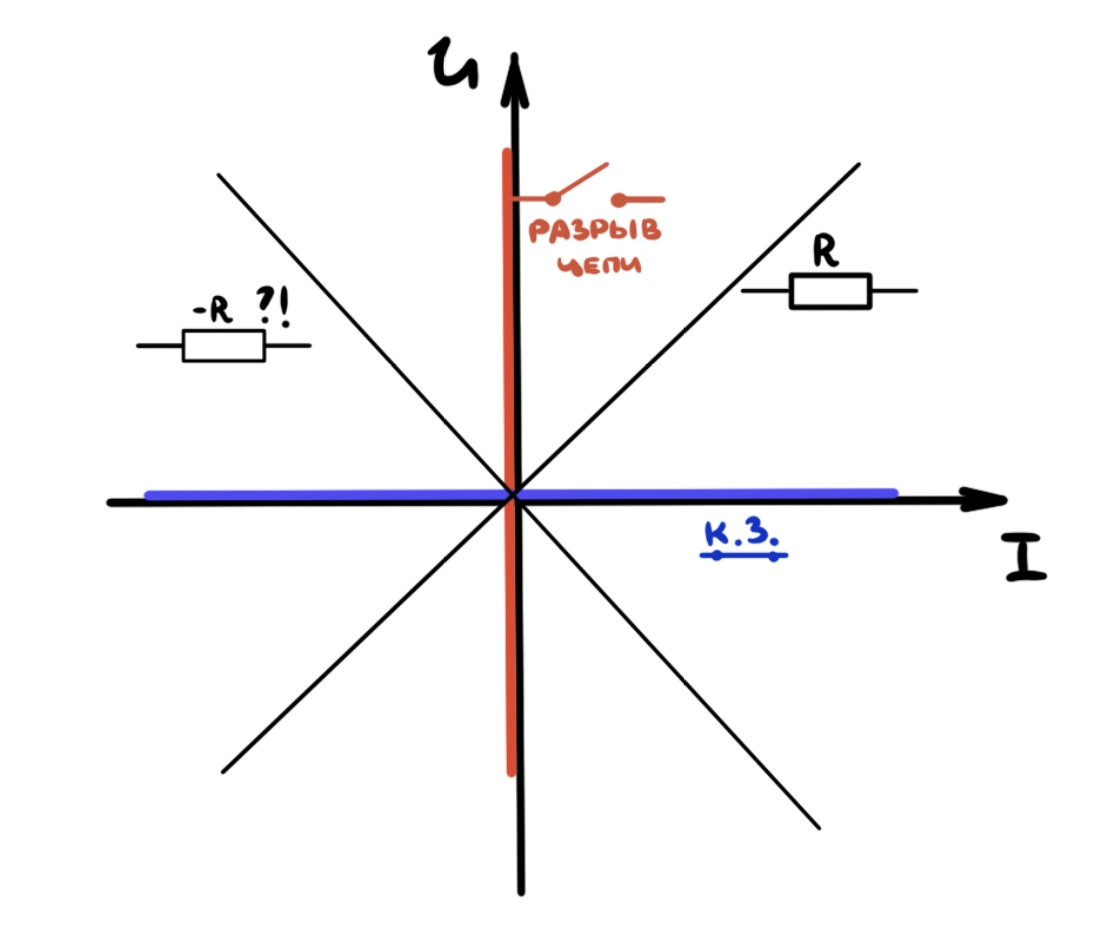
\includegraphics[width=0.5\textwidth]{Images/Capture_20250906_005642.jpg}
    \caption{Пассивные двухполюсники}
    \label{fig:Capture_20250906_005642}
\end{figure}
Все эти двухполюсники являются пассивными, они не могут сами генерировать электрический ток, 
поэтому чтобы в нашей цепи потек ток, мы должны выйти за границы линейных двухполюсников.
\section*{Аффинные двухполюсники}
Если вы еще не забыли курс линейной алгебры, то должны помнить, что в нем рассматривались 
линейные и аффинные преобразования. Аффинные преобразования можно было представить в виде 
двух последовательно действующих преобразований, одно из которых - это некоторое линейное 
преобразование, а второе - преобразование сдвига (или трансляции).
В случае с аффинным двухполюсником аналогия со сдвигом сохраняется. По сути аффинный 
двухполюсник получается сдвигом множества состояний линейного двухполюсника на некоторый 
вектор. Таким сдвигом из пассивных элементов мы получим источники.
\begin{figure}[h!]
    \centering
    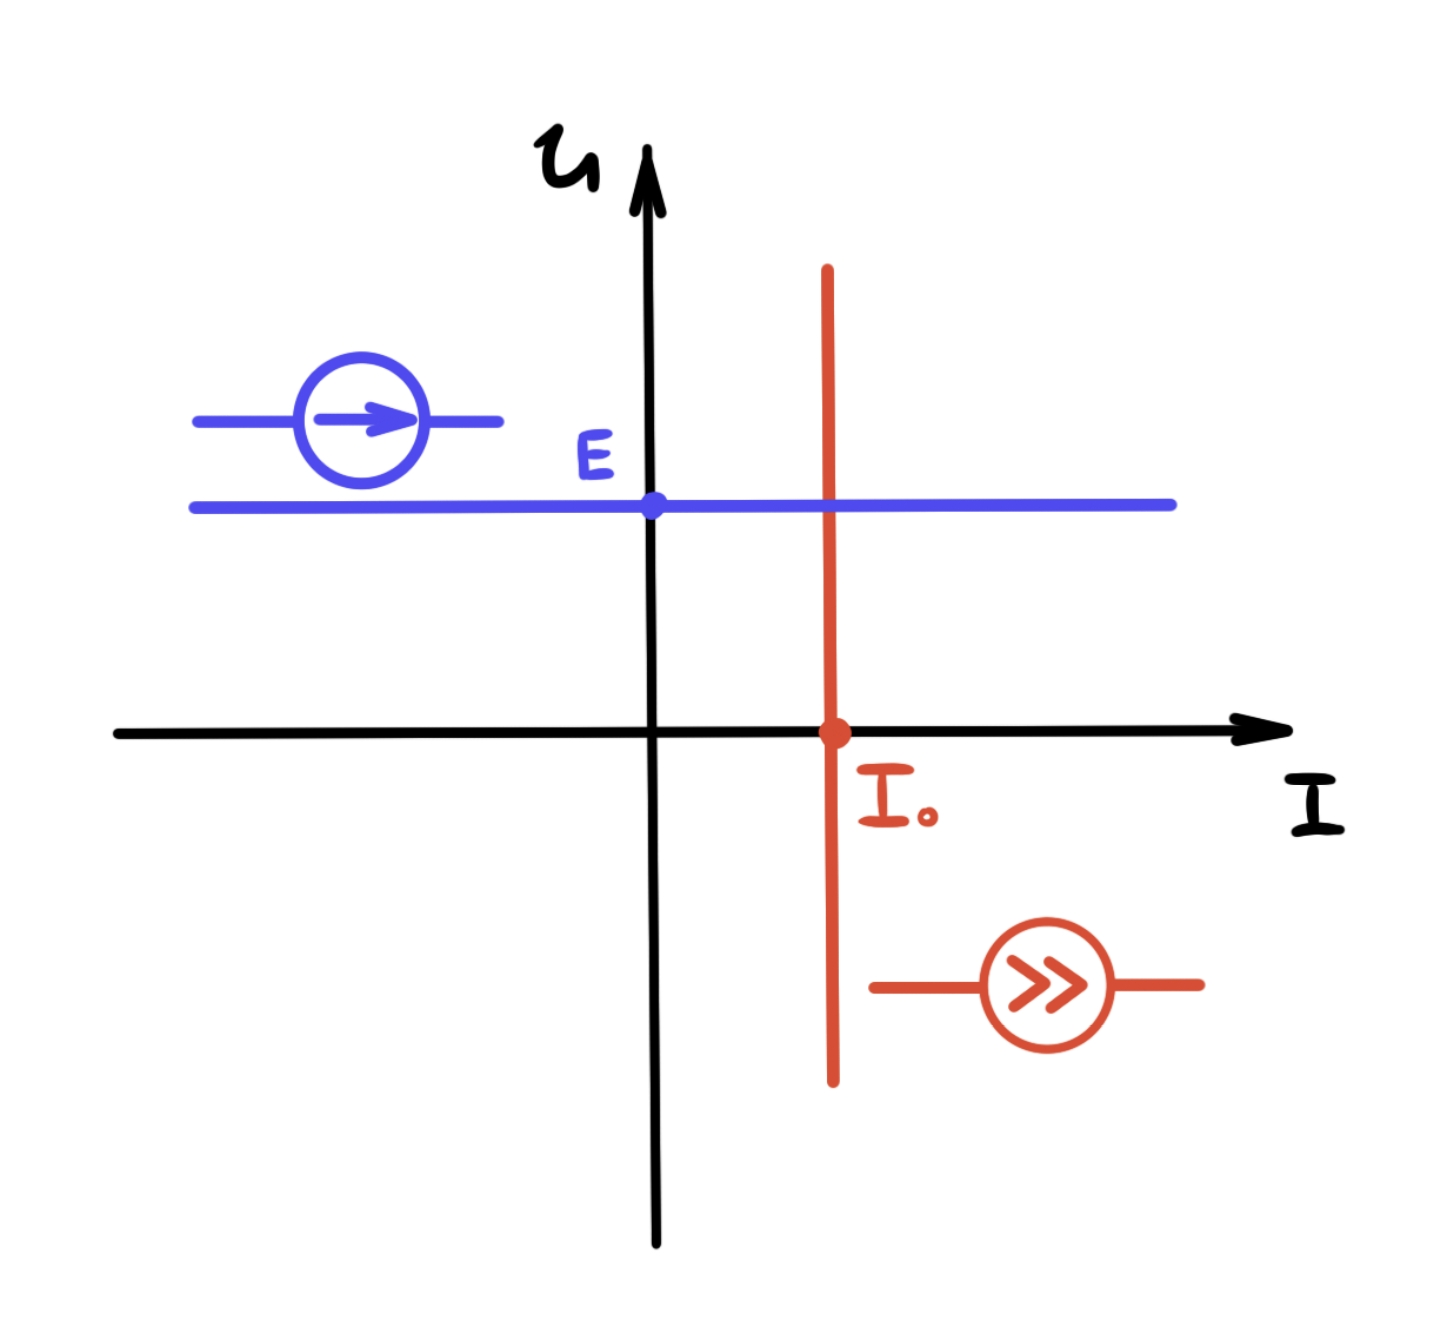
\includegraphics[width=0.4\textwidth]{Images/ideal_sources.jpg}
    \caption{Идеальные источники}
    \label{fig:ideal_sources}
\end{figure}
Например если мы сдвинем горизонтальную прямую, соответствующую разрыву цепи, то получим 
идеальный источник тока, так как теперь множество состояний двухполюсника таково, что любому 
значению напряжения соответствует один ток. Если мы сдвинем вертикальную прямую из нулевого 
положения, соответствующего короткому замыканию, то получим идеальный источник напряжения, 
так как для любого потребляемого тока этот двухполюсник будет выдавать постоянную разницу потенциалов. 
Проблема в том, что такие источники являются идеальной моделью, которая не реализуется на практике.

\subsection*{Реальные источники}
Если вы когда нибудь работали с электрическими цепями и подключали их к источникам энергии (аккумуляторам или батарейкам), то должны были заметить, что напряжение на источнике при подключении внешней цепи ``проседает''. Обсудим, почему это проиcходит.
Если исключить вырожденные случаи, рассмотренные выше, то аффинный двухполюсник задается наклонной прямой, которая пересекается в одной точке с осью ординат, а в другой - с осью абсцисс. Эта прямая будет задавать так называемый ``реальный источник''. Пересечение с горизонтальной осью соответствует случаю с нулевым напряжением - то есть состоянию короткого замыкания. Пересечение с вертикальной осью - случаю с нулевым током, то есть состоянию холостого, хода, когда источник ни к чему не подключен.
\begin{figure}[h!]
    \centering
    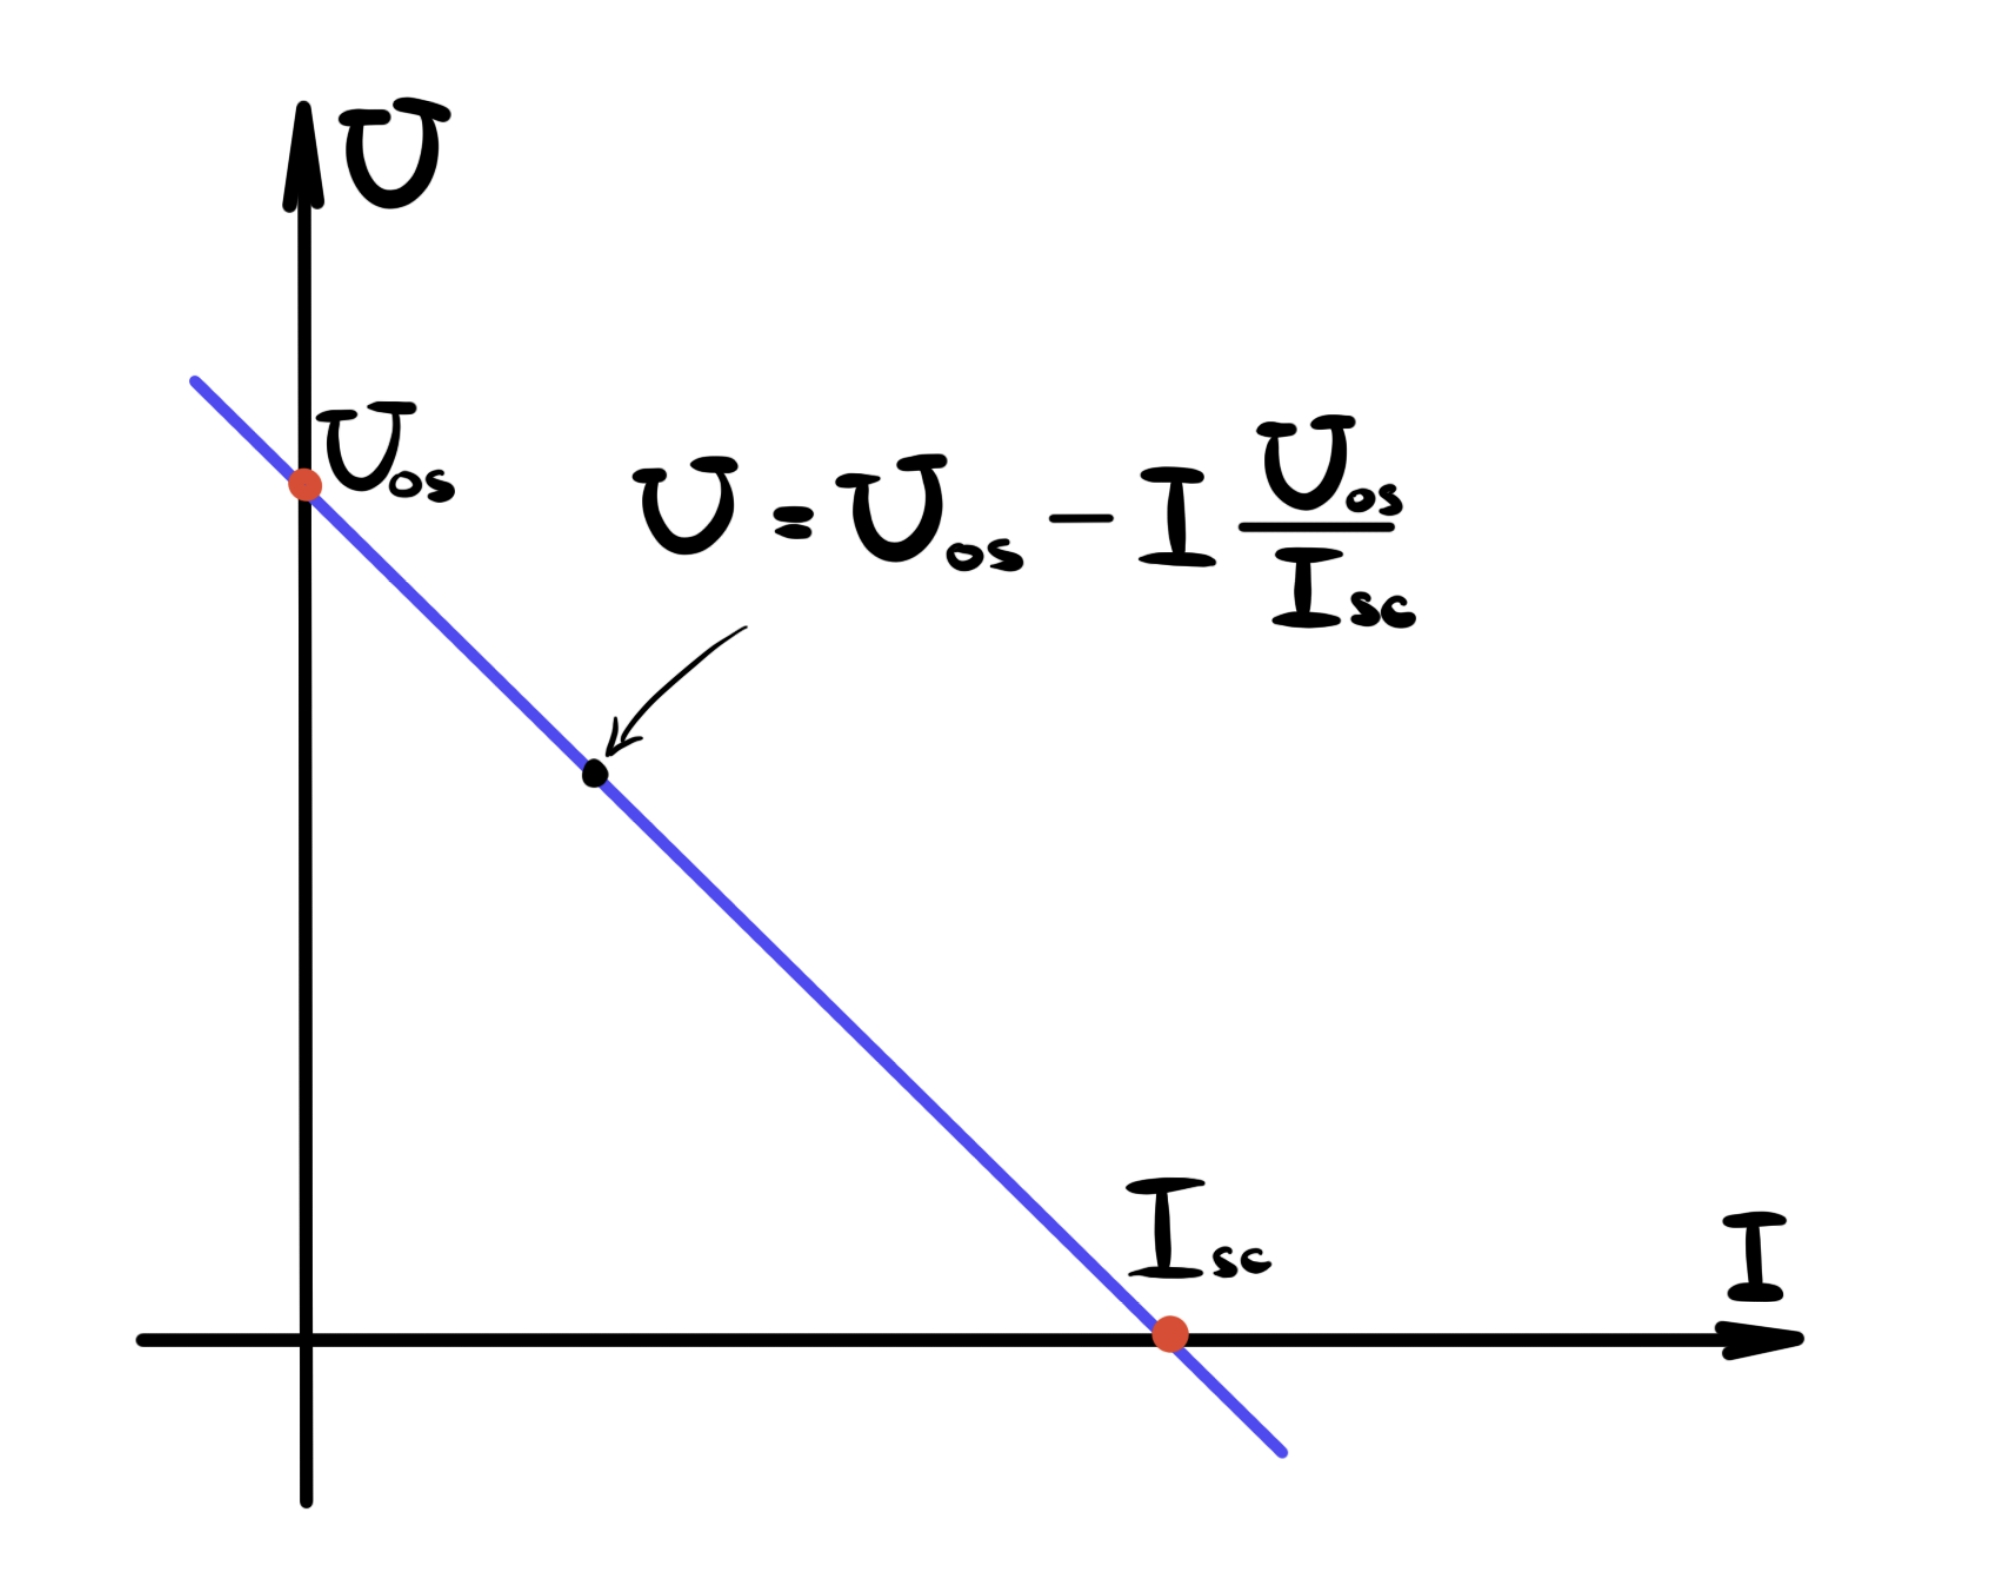
\includegraphics[width=0.5\textwidth]{Images/real_source.jpg}
    \caption{Реальный источник}
    \label{fig:real_source}
\end{figure}
Таким образом, если у нас есть источник, то мы можем измерить ток короткого замыкания $I_{sc}$ (short circuit) и напряжение холостого хода $U_{os}$ (open circuit). Эти две величины определяют уравнение задающее наклонную прямую.
$$
U = E - IR = U_{os} - I \frac{U_{os}}{I_{sc}}
$$
Из формулы становится ясно: если источник, с которым мы работаем, описывается линейной моделью реального двухполюсника, то при подключении такого источника в цепь, через него потечет ток, а значит состояние сместится из точки холостого хода, следовательно напряжение получившегося состояния окажется меньше. В этом и кроется причина ``проседания'' напряжения.
\subsection*{Теорема Тевенена}
Оказывается, если мы подключим последовательно идеальный источник напряжения и резистор, то на выходе получившегося двухполюсника получим похожую наклонную прямую. Связь между напряжением и силой тока в таком двухполюснике будет задаваться следующим линейным уравнением.
$$
U = E - IR
$$
Значит, если мы возьмем идеальный источник с напряжением $E = U_{os}$ и сопротивлением $R = \frac{U_{os}}{I_{sc}}$, то получим модель, которая ведет себя также, как и наш неидеальный источник. Таким образом мы явно показали, как можно заменить подобной схемой аффинный двухполюсник. Это суть теоремы Тевенена
\begin{figure}[h!]
    \centering
    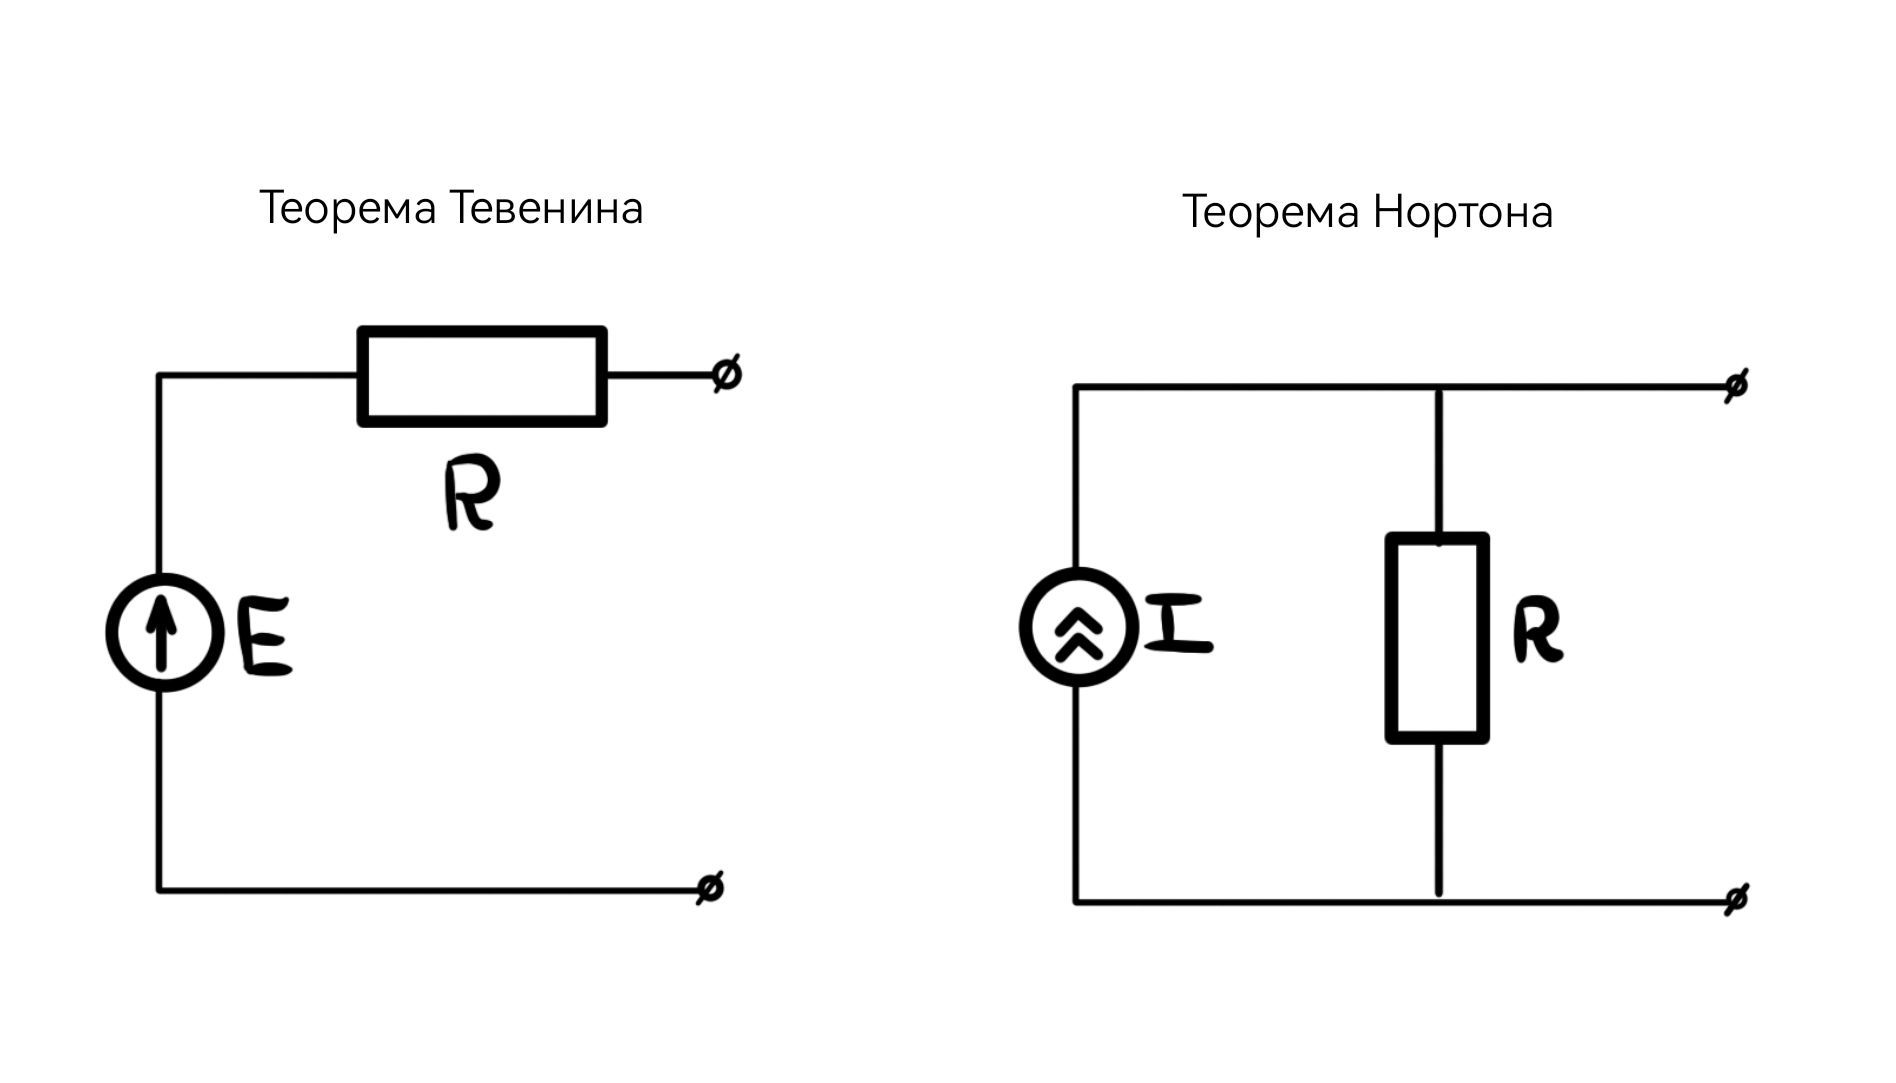
\includegraphics[width=0.9\textwidth]{Images/tevenin_i_norton.jpg}
    \caption{Теоремы Тевенена и Нортона}
    \label{fig:tevenin_i_norton}
\end{figure}
\subsection*{Теорема Нортона}
С другой стороны можно сконструировать двухполюсник подключив параллельно сопротивление $R$ c идеальным источником тока $I_0$. Уравнение описывающее такой двухполюсник имеет вид:
$$
I_0 = I + \frac{U}{R} \quad \Rightarrow \quad U = I_0R - IR
$$
Значит для получения такой модели исходного аффинного двухполюсника, параметры цепочки должны быть такими:
$$
U_{oc} = I_0R; \quad R = \frac{U_{oc}}{I_{sc}} \Rightarrow I_0 = I_{sc}
$$
Так, мы явно показали, как можно заменить аффинный двухполюсник моделью с идеальным источником. Это суть теоремы Нортона.

\subsection*{Применимость теорем}
Аффинный источник можно представить любым из предложенных способов. Так каким же пользоваться? Положа руку на сердце, каждый сказал бы, что удобнее пользоваться теоремой Тевенена, поскольку работать с идеальным источником напряжения мы привыкли со школы, однако это удобно не всегда.
Есть такое понятие как нагрузка (load) и сопротивление нагрузки $R_l$.
Нагрузка - это нечто, что мы подключаем к нашему двухполюснику. Лампочка, двигатель, усилитель и так далее. Сопротивление нагрузки - это сопротивление эквивалентного резистора, который установит наш источник в такое же состояние, что и нагрузка.
Если сопротивление нагрузки сильно больше внутреннего сопротивления источника $R \ll R_l$, ток через нагрузку почти не потечёт и напряжение на выходе двухполюсника почти не будет зависеть от нагрузки, а значит источник будет похож на идеальный источник напряжения
Если наоборот $R \gg R_l$ то почти весь ток потечет через нагрузку и поведение двухполюсника будет близко к поведению идеального источника тока.В таком случае уже удобно воспользоваться теоремой Нортона.

\section*{Делитель напряжения}
Ярким примером аффинного двухполюсника, является делитель напряжения. Из названия понятно, что такое схемное решение нужно для того, чтобы поделить напряжение. Представьте ситуацию, что у вас есть аккумулятор на 3.6 вольт, и вам нужно запитать от него микроконтроллер, который поддерживает 2.4 вольта. Для решения этой проблемы попробуем применить наш делитель.
\begin{figure}[h!]
    \centering
    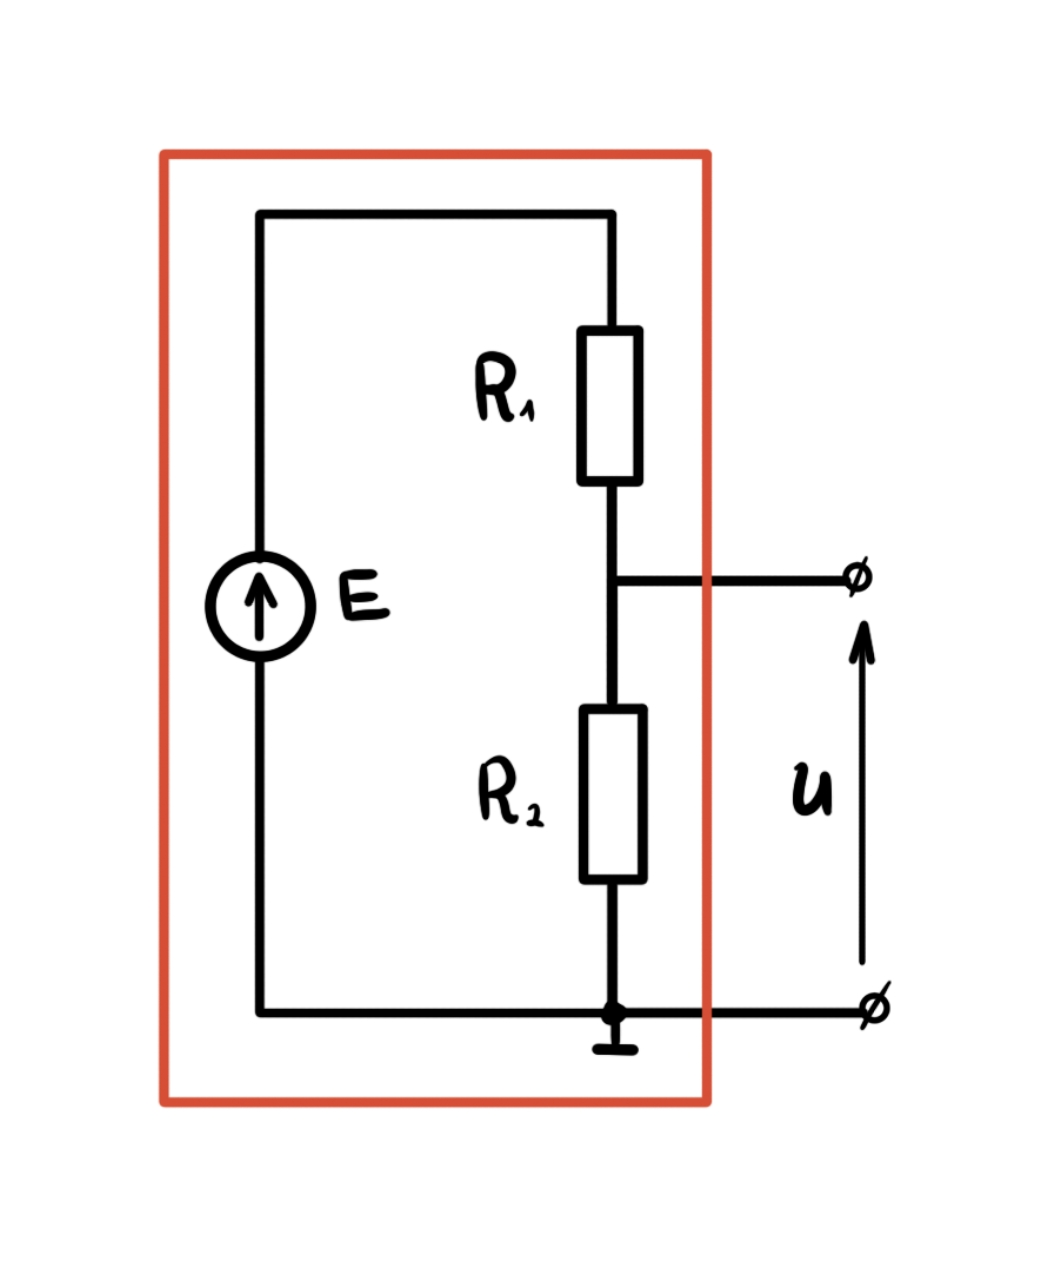
\includegraphics[width=0.4\textwidth]{Images/delitel_1.jpg}
    \caption{Делитель напряжения}
    \label{fig:delitel_1}
\end{figure}
Итак, чтобы найти уравнение прямой для этого двухполюсника, найдем напряжение холостого хода. Для этого оставим цепь разомкнутой. Остается лишь один контур, по которому течет ток $I$.
$$
I = \frac{E}{R_1 + R_2} \Rightarrow U_{oc} = IR_2 = \frac{R_2}{R_1 + R_2}E
$$
Теперь устроим на выходе короткое замыкание. Ток не будет течь по резистору $R_2$: $I_{sc} = \frac{E}{R_1}$. Уравнение прямой:
$$
U = U_{oc} - I\frac{U_{oc}}{I_{sc}}\quad \Rightarrow \quad U = \frac{R_2}{R_1+R_2}E - I\frac{R_1R_2}{R_1+R_2}
$$
Теперь применим теорему Тевенена и получим напряжение и внутреннее сопротивление эквивалентного источника.
$$
E^* = \frac{R_2}{R_1+R_2}E; \quad R^* = \frac{R_1R_2}{R_1+R_2} = R_1||R_2
$$
\begin{figure}[h!]
    \centering
    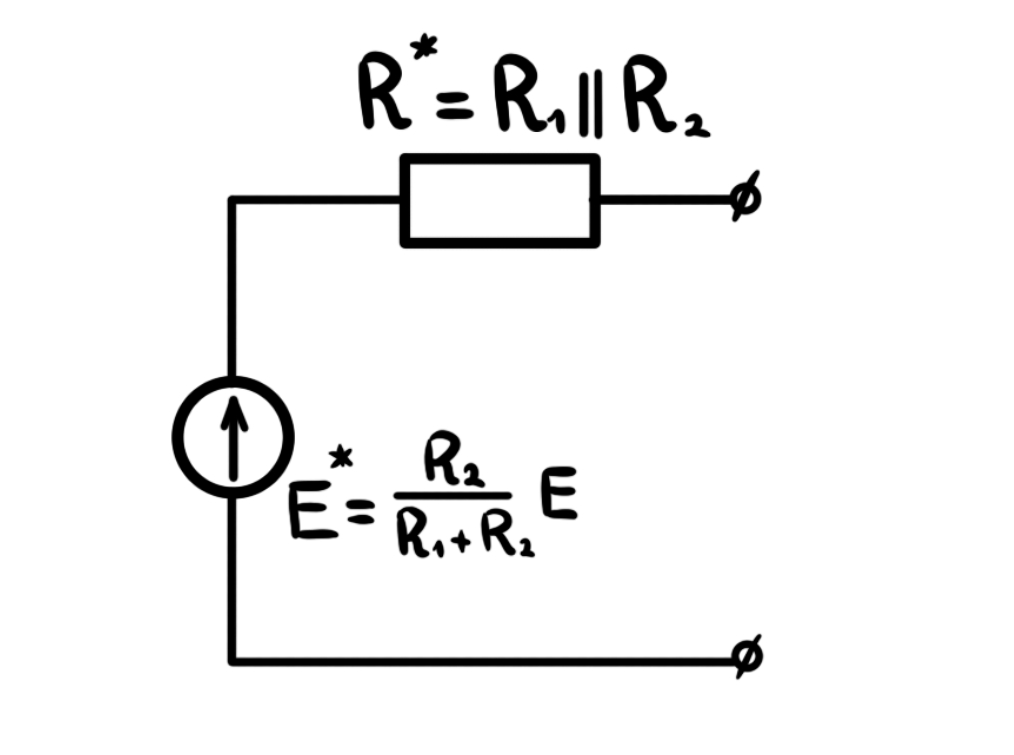
\includegraphics[width=0.6\textwidth]{Images/delitel_2.jpg}
    \caption{Эквивалентная схема делителя напряжения}
    \label{fig:delitel_2}
\end{figure}
Заметим, что если у нашего исходного аккумулятора было маленькое внутреннее сопротивление и напряжение при 
подключении нагрузки почти не падало, то у получившегося источника внутреннее сопротивление определяется резисторами 
$R_1$ и $R_2$. Если эти сопротивления не будут достаточно маленькими, то при подключении к нагрузки, напряжение на 
нем может сильно проседать. С другой стороны, сколь угодно малыми их тоже нельзя делать, потому что в такое случае в 
режиме холостого хода будет рассеиваться большая мощность. Таким образом делитель напряжения не всегда является удачным схемным решением.
\section*{Параллельный сумматор}
Параллельный сумматор довольно часто возникает возникает в схемных решениях не по воле инженера, а скорее спонтанно. 
Например в вы столкнетесь с ним в следующем семестре, когда будете изучать усилители с обратными связями.
\begin{figure}[h!]
    \centering
    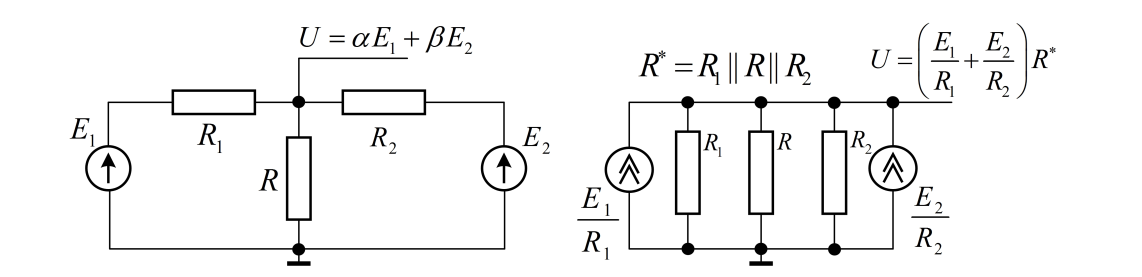
\includegraphics[width=1\textwidth]{Images/summator_1.png}
    \caption{Параллельный сумматор}
    \label{fig:summator_1}
\end{figure}
Допустим у нас заданы коэффициенты $\alpha$ и $\beta$, с которыми должны складываться напряжения источников. Наша 
задача - подобрать сопротивления. Соотношение $U = \alpha E_1 + \beta E_2$ должно работать при любых напряжениях источников. 
Тогда мы можем заменить источник $E_2$ на короткое замыкание. Рассчитаем схему для этого случая. На самом деле легче разглядеть 
здесь делитель напряжения, представив параллельно подключенные $R$ и $R_2$ одним эквивалентным резистором. Получим 
$U = \frac{R||R_2}{R_1 + R||R_2}E_1$. Отсюда $\alpha = \frac{R||R_2}{R_1 + R||R_2}$. Симметрично приравняв к нулю левый 
источник получим $\beta = \frac{R||R_1}{R_2 + R||R_1}$.
Связь мы нашли, однако непонятно, как отсюда выразить искомые сопротивления.
Время для финта ушами. Если посмотреть на отдельно ветвь, состоящую из напряжения $E_1$ и резистора $R_1$, то можно разглядеть 
эквивалентный источник из теоремы Тевенена. Однако замена с помощью теоремы Тевенена и теоремы Нортона равнозначны, мы можем 
воспользоваться любой, тогда этот аффинный двухполюсник можно представить как параллельно подключенные источник тока и сопротивление. 
Теперь заменим параллельно подключенные источники одним эквивалентным с сопротивлением $R^* = R_1||R||R_2$. Параллельно подключенные 
источники также можно заменить одним источником с постоянным током $\frac{E_1}{R_1} + \frac{E_2}{R_2}$. Теперь можно выразить напряжение 
на выходе сумматора: $U = R^*(\frac{E_1}{R_1} + \frac{E_2}{R_2})$
Путем сравнения с исходной формулой получаем:
$$
\begin{array}{l}
\alpha = \frac{R^*}{R_1} \\ \beta = \frac{R^*}{R_2}
\end{array} \quad\Rightarrow\quad
\frac{\alpha}{\beta} = \frac{R_2}{R_1}
$$
Для нахождения сопротивлений по заданным $\alpha$ и $\beta$ нам нужно еще одно соотношение.
$$
\alpha + \beta = R^* \left(\frac{1}{R_1}+ \frac{1}{R_2}\right) = \frac{(R_1||R_2)||R}{R_1||R_2}
$$
Для удобства сделаем временную замену: $r = R_1 || R_2$.
$$
\frac{r||R}{r} = \frac{rR}{r(R+r)} = \frac{1}{1 + \frac{r}{R}} = \frac{1}{1+ \frac{R_1+ R_2}{R}}
$$
Сопротивления у нас три, а формулы всего две, поэтому одни из напряжений мы можем выбрать.
\section*{Линейные трёхполюсники}
Если у нашего черного ящика появляется еще один выход, ситуация усложняется. Для описания его состояния нужно уже шесть
параметров: потенциал каждого полюса $\varphi_1, \; \varphi_2, \; \varphi_3, \;$ и ток, протекающий через каждый полюс 
$I_1, \; I_2, \; I_3$.
Один из полюсов как правило называют общим. (По сути этот полюс выступает в роли земли и все потенциалы считаются от него). 
Назовем общим третий полюс.
\begin{figure}[h!]
    \centering
    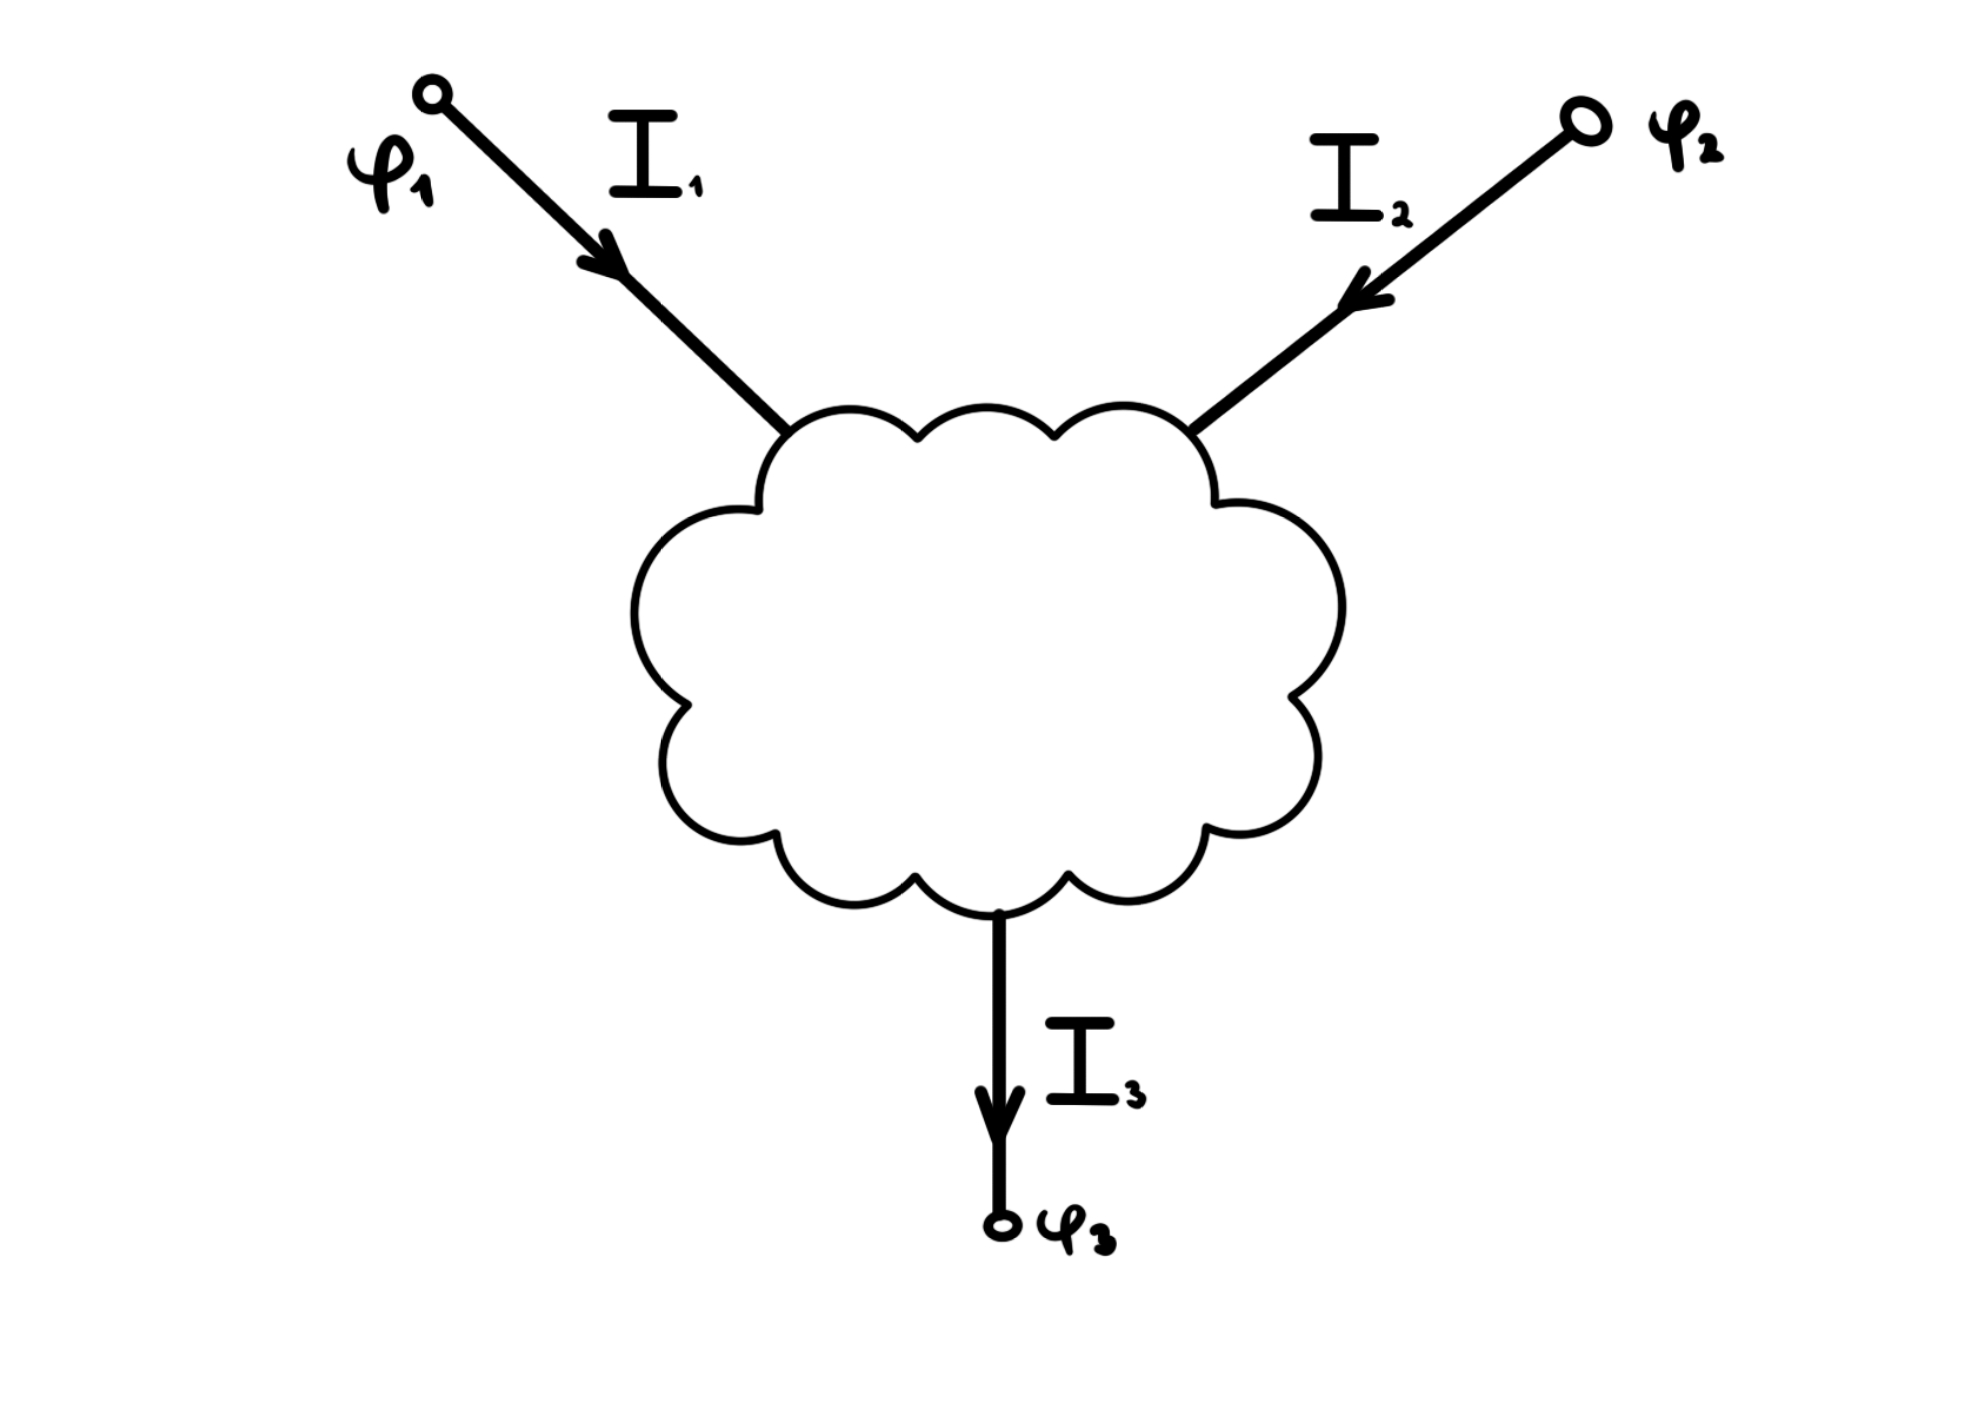
\includegraphics[width=0.4\textwidth]{Images/3_polus.jpg}
    \caption{Трехполюсник}
    \label{fig:3_polus}
\end{figure}
Трехполюсник не может накапливать заряд, если он является безынерционным, поэтому один ток будет выражаться через остальные. 
Выразим ток, вытекающий из общего полюса: $I_3 = I_1 + I_2$.

А еще можно от потенциалов перейти к напряжениям относительно третьего полюса: 
$U_1 = \varphi_1 - \varphi_3; \quad U_2 = \varphi_2 - \varphi_3$. Таким образом от шести переменных 
мы перешли к четырем: $(U_1, U_2, I_1, I_2)$.
Обобщив один из полюсов и сделав замену параметров, мы на самом деле перешли от трехполюсника к 
рассмотрению четырехполюсника, где общий полюс образует с каждым оставшимся полюсом пару, так называемый \textbf{порт}. 
Далee будем называть исследуемый объект \textbf{четырехполюсником}.

Итак если четырехполюсник линеен, то линейное пространство его состояний является подпространством в 
\textbf{четырехмерном векторном пространстве}. (В то время как у двухполюсника это пространство было всего двумерным) 
Какова размерность этого подпространства? Если не рассматривать вырожденные случаи, то обычно в четырехполюсниках возникнет 
две линейные связи, которые уменьшат размерность нашего линейного пространства до двух. Далее рассматриваем четырехполюсники 
с двумерным линейным пространством состояний.

\subsection*{Флэшбек из аналитической геометрии}
Обратимся к курсу аналитической геометрии. Там, чтобы задать прямую в трехмерном пространстве, мы представляли ее как 
пересечение двух неколлинеарных плоскостей. Сами же плоскости мы задавали через их вектора нормали.
\begin{figure}[h!]
    \centering
    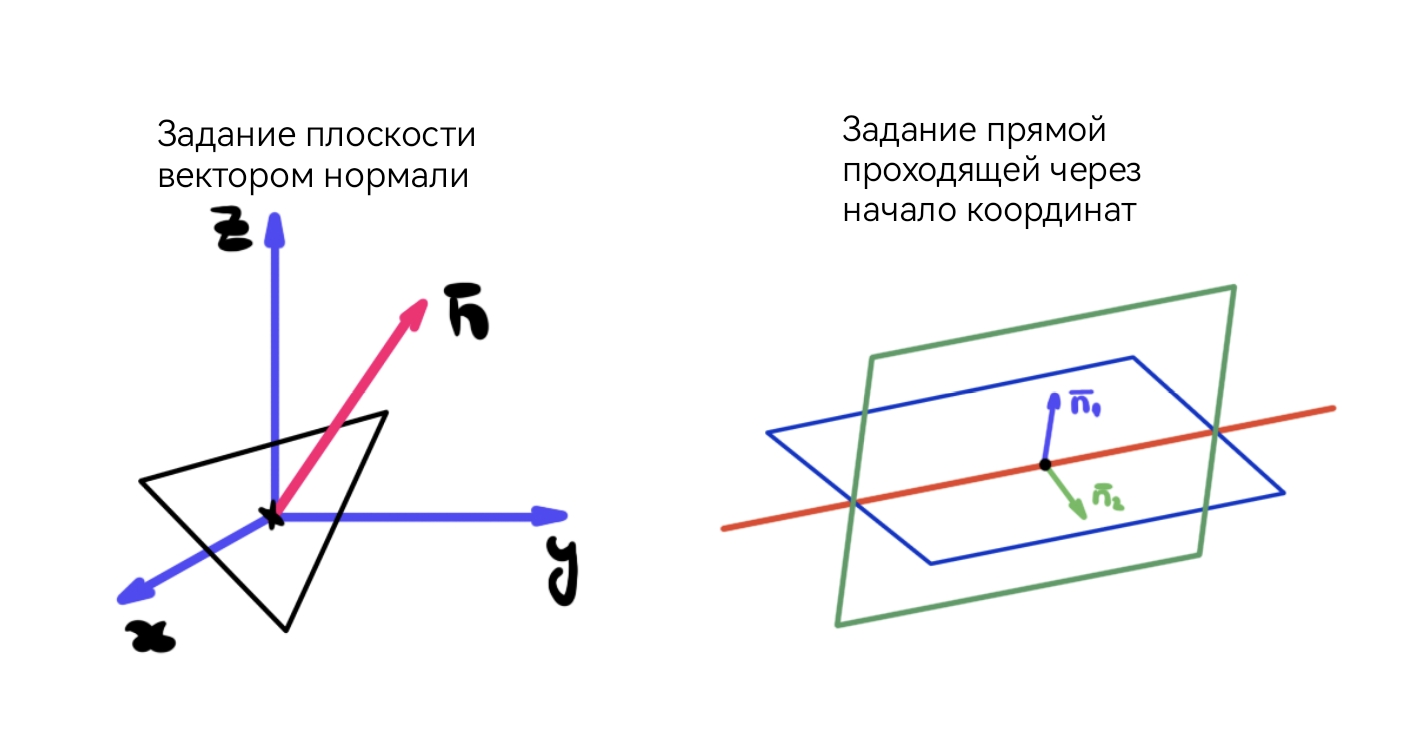
\includegraphics[width=0.9\textwidth]{Images/ploskosti.jpg}
    \caption{Пересечение плоскостей}
    \label{fig:ploskosti}
\end{figure}
Если плоскость проходит через начало координат(линейное пространство), то задать ее довольно просто.
$$
(\overline{n}, \overline{x})= n_xx + n_yy + n_zz = 0
$$
Таким образом задание прямой сводилось к паре линейных уравнений
$$
\begin{cases}
a_1x + b_1y + c_1z = 0 \\
a_2x + b_2y + c_2z = 0 \\
\end{cases}
$$
Мы же имеем дело с четырехмерным пространством, поэтому размерность повышается: в нашем случае мы задаем двумерное 
линейное пространство как пересечение двух трехмерных \textbf{гиперплоскостей}, которые в свою очередь задаются двумя 
четрырехмерными векторами нормали: 
$\overline{n_1}= (\alpha_1, \beta_1, \gamma_1, \delta_1)$, $\overline{n_2}= (\alpha_2, \beta_2, \gamma_2, \delta_2)$ 
а соответствующая система уравнений примет вид:
$$
\begin{cases}
\alpha_1U_1 + \beta_1U_2 + \gamma_1I_1 + \delta_1I_2 = 0 \\
\alpha_2U_1 + \beta_2U_2 + \gamma_2I_1 + \delta_2I_2 = 0 \\
\end{cases}
$$
Когда мы решаем эту систему уравнений в общем виде, мы выражаем одну пару переменных через другую пару. Сделать это можно 
шестью разными способами.
Не всегда удается выразить одну пару переменных через другую, но один из шести способов всегда сработает, так как иначе 
уравнения были бы линейно зависимы, и следовательно двухполюсник имел бы трехмерное пространство состояний или еще того 
хуже - нульмерное.

Рассмотрим общую теорию на важном частном случае.
\subsection*{h-параметры}
h-параметры это cпособ выражения величин трехполюсника, который часто используется в усилительной технике. В нем входное 
напряжение $U_1$ и выходной ток $I_2$ выражаются через $U_2$ и $I_1$. Запишем исходную систему в более удобном виде и 
преобразуем к матричному виду.
$$
\begin{cases}
\alpha_1U_1 + \delta_1I_2 = -\gamma_1I_1 -\beta_1U_2 \\
\alpha_2U_1 + \delta_2I_2 = -\gamma_2I_1 -\beta_2U_2 \\
\end{cases}
\; \Leftrightarrow \;
\begin{pmatrix}
\alpha_1 & \delta_1 \\ \alpha_2 & \delta_2\\
\end{pmatrix}
\begin{pmatrix} U_1\\ I_2\\\end{pmatrix}
=-
\begin{pmatrix}
\gamma_1 & \beta_1 \\ \gamma_2 & \beta_2\\
\end{pmatrix}
\begin{pmatrix} I_1\\ U_2\\\end{pmatrix}
$$
Если матрица $(\alpha \; \delta)$ окажется невырожденной, то можнно домножить обе части равенства слева на обратную к ней матрицу.
$$
\begin{pmatrix} U_1\\ I_2\\\end{pmatrix}
=-
\begin{pmatrix}
\alpha_1 & \delta_1 \\ \alpha_2 & \delta_2\\
\end{pmatrix}^{-1}
\begin{pmatrix}
\gamma_1 & \beta_1 \\ \gamma_2 & \beta_2\\
\end{pmatrix}
\begin{pmatrix} I_1\\ U_2\\\end{pmatrix}
$$
Полученная таким образом матрица называется \textbf{матрицей h-параметров}.
$$
\begin{pmatrix} U_1\\ I_2\\\end{pmatrix}
=
\begin{pmatrix}
h_{11} & h_{12} \\ h_{21} & h_{22}\\
\end{pmatrix}
\begin{pmatrix} I_1\\ U_2\\\end{pmatrix}
$$
Если матрица $(\alpha \; \delta)$ окажется вырожденной, это значит, что переменные $I_1$ и $U_2$
являются зависимыми, и h-параметры для описания этой системы не подходят.

Попробуем понять смысл каждого параметра. Для этого перейдем от матричного 
вида к системе и изобразим эквивалентную схему.
$$
\begin{array}{l}
U_1 = h_{11}I_1 + h_{12}U_2 \\
I_2 = h_{21}I_1 + h_{22}U_2 \\
\end{array}
$$
\begin{figure}[h!]
    \centering
    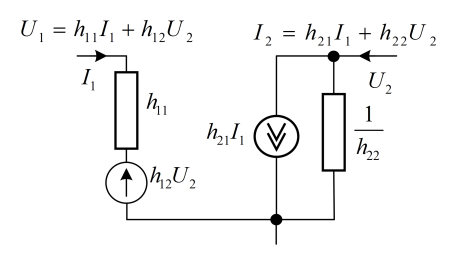
\includegraphics[width=0.7\textwidth]{Images/h_parameters.png}
    \caption{Эквивалентная схема с h-параметрами}
    \label{fig:h_parameters}
\end{figure}
Из первого уравнения видно, что $h_{11}$ имеет размерность сопротивления, $h_{12}$ - безразмерный коэффициент. 
Таким образом первое уравнение можно реализовать последовательно соединенными резистором с сопротивлением $R$ 
и новым элементом, который назыается \textbf{управляемым источником напряжения}.
Из второго уравнения видно, что $h_{21}$ безразмерный, $h_{22}$ имеет размерность проводимости. Второе уравнение можно раелилзовать паралленьно 
соединенным \textbf{управляемым источником тока} и резистором. Все это мы подключaем к общему третьему полюсу (земле). 
Эта модель четырехполюсника будет вести себя точно также, как и модель, задающаяся уравнениями на $U_1$ и $I_2$.
\subsection*{T-образная схема}
Чтобы понять, как приводить трехполюсники к модели h-параметров, рассмотрим пример из вашего задания. 
Найдем h-параметры Т-образной схемы.
\begin{figure}[h!]
    \centering
    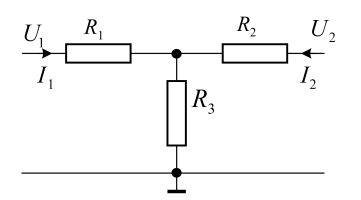
\includegraphics[width=0.5\textwidth]{Images/T_scheme_0.png}
    \caption{Т-образная схема}
    \label{fig:T_scheme_1}
\end{figure}
Исключим из уравнений $U_2$. Для этого ``закоротим'' выходной порт. А на вход подадим ток $I_1 = I_0$. 
Уравнения на h-параметры упростились:
$$
\begin{array}{l}
U_1 = h_{11}I_0 \\
I_2 = h_{21}I_0 \\
\end{array}
$$
$U_1 = (R_1 + R_2 || R_3)I_0$ 
Теперь найдем связь $U_1$ в получившейся схеме. 
Сравнивая получившееся с первым уравнением системы получаем $h_{11} = R_1 + R_2 || R_3$. Для нахождения 
тока введем вспомогательные переменные (см. рис. ниже).
\begin{figure}[h]
    \centering
    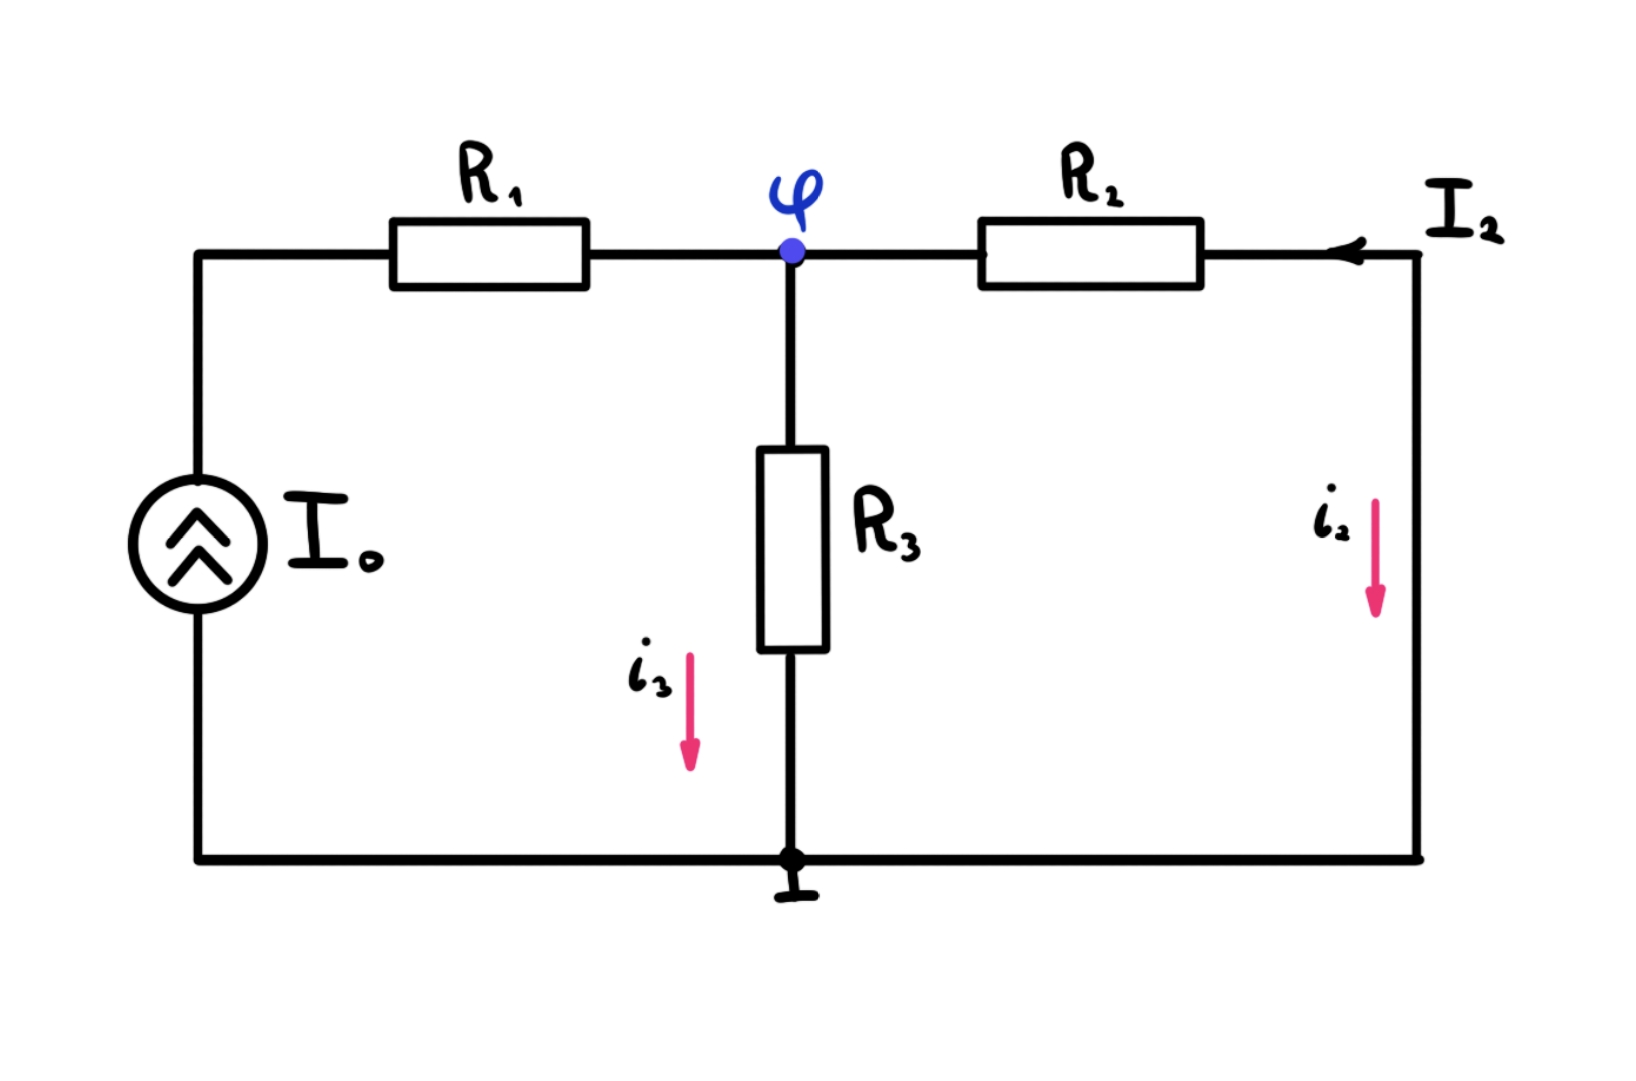
\includegraphics[width=0.4\textwidth]{Images/T_scheme.jpg}
    \caption{Расчет T-образной схемы}
    \label{fig:T_scheme_2}
\end{figure}
$$
\begin{array}{l}
i_2 + i_3 = I_0 \\
\varphi = i_3R_3 = i_2R_2
\end{array} \Rightarrow
i_2 = I_0 \frac{1}{1 + R_2/R_3} = I_0 \frac{R_3}{R_3 + R_2}
$$
$$
I_2 = -i_2 = - I_0 \frac{R_3}{R_3 + R_2}
$$
Сравнивая со вторым уравнением системы получаем: $$h_{21} = -\frac{R_3}{R_3 + R_2}$$
Для нахождения второй пары параметров избавимся от ослагаемых с $I_1$ на входе. Для этого оставим входной порт
разомкнутым а на выходной 
порт подадим напряжение $U_0$ с помощью идеального источника.
\begin{figure}[h!]
    \centering
    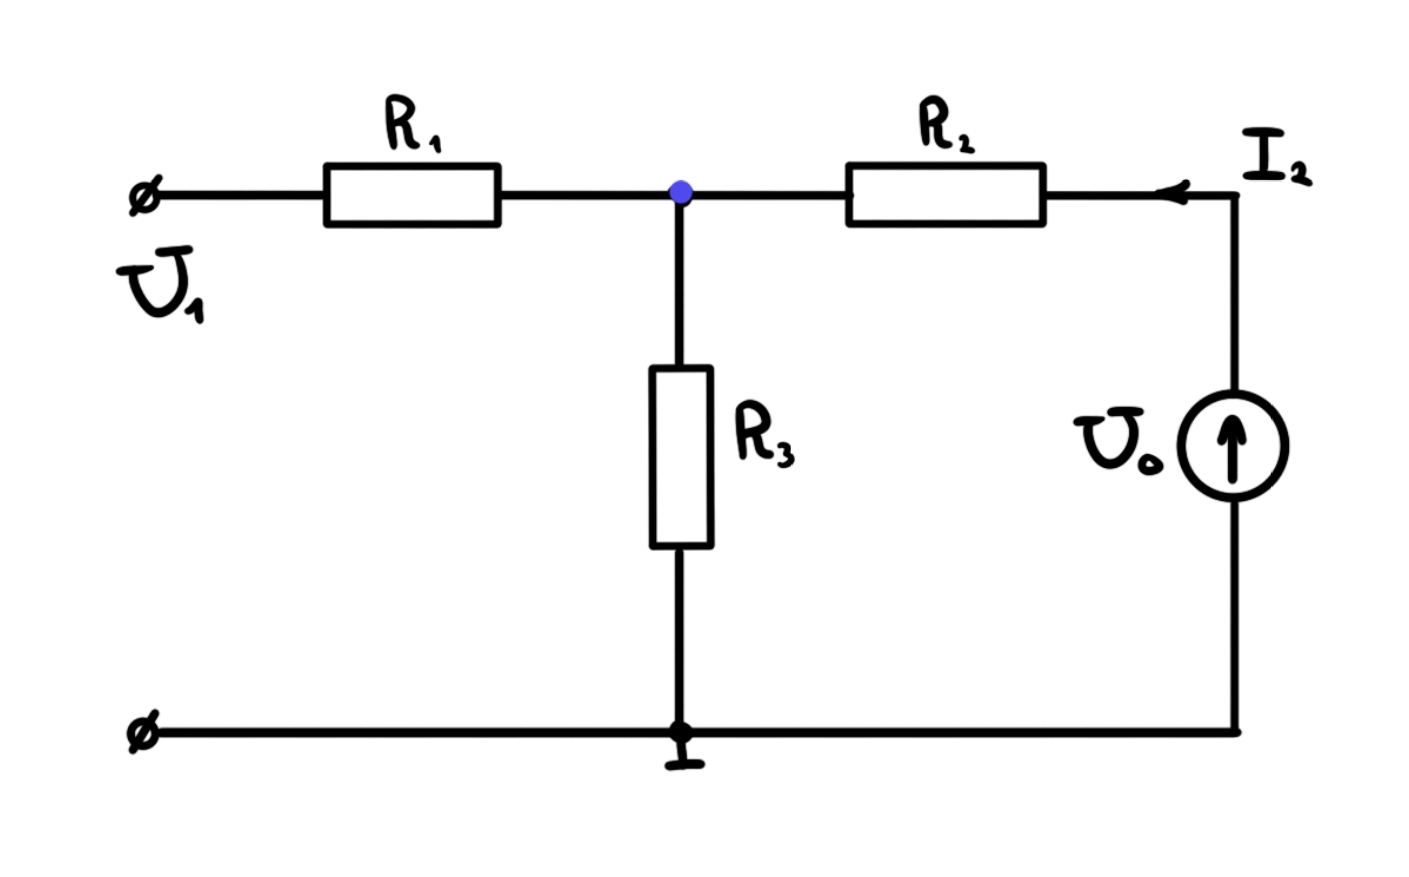
\includegraphics[width=0.4\textwidth]{Images/T_scheme_2.jpg}
    \caption{Расчет T-образной схемы (2)}
    \label{fig:T_scheme_3}
\end{figure}
Уравнения упростились:
$$
\begin{array}{l} 
U_1 = h_{12}U_0 \\
I_2 = h_{22}U_0 \\
\end{array}
$$
Получим соответствующие связи в схеме. Ток $I_2$ от источника напряжения течет через резисторы $R_2$ и $R_3$, на 
резисторе $R_1$ падения напряжения нет, так как ток через него не течет, следовательно: $I_2(R_2 + R_3) = U_0$. Сравнивая 
со вторым уравнением системы получаем:
$$h_{22} = \frac{1}{R_2 + R_3}$$
Потенциал $U_1$ равен потенциалу в единственном узле:
$$
U_1 = R_3 I_2 = \frac{R_3}{R_2 + R_3}U_0\;\Rightarrow \; h_{12} = \frac{R_3}{R_2 + R_3}
$$
Запишем получившуюся матрицу h-параметров.
$$
\begin{pmatrix} U_1\\ I_2\\\end{pmatrix}
=
\begin{pmatrix}
R_1 + R_2 || R_3 & \frac{R_3}{R_2 + R_3} \\ -\frac{R_3}{R_3 + R_2} & \frac{1}{R_2 + R_3}\\
\end{pmatrix}
\begin{pmatrix} I_1\\ U_2\\\end{pmatrix}
$$
\subsection*{X-параметры и Y-параметры}
Еще два способа описания линейного четырехполюсника. X-пармаетры выражают напряжения через токи, а Y-парметры -- наоборот:
$$
\begin{pmatrix} U_1\\ U_2\\\end{pmatrix}
=
\begin{pmatrix}
X_{11} & X_{12} \\ X_{21} & X_{22}\\
\end{pmatrix}
\begin{pmatrix} I_1\\ I_2\\\end{pmatrix}
; \quad
\begin{pmatrix} I_1\\ I_2\\\end{pmatrix}
=
\begin{pmatrix}
Y_{11} & Y_{12} \\ Y_{21} & Y_{22}\\
\end{pmatrix}
\begin{pmatrix} U_1\\ U_2\\\end{pmatrix}
$$
На рисунке представлены их эквивалентные модели.
\begin{figure}[h!]
    \centering
    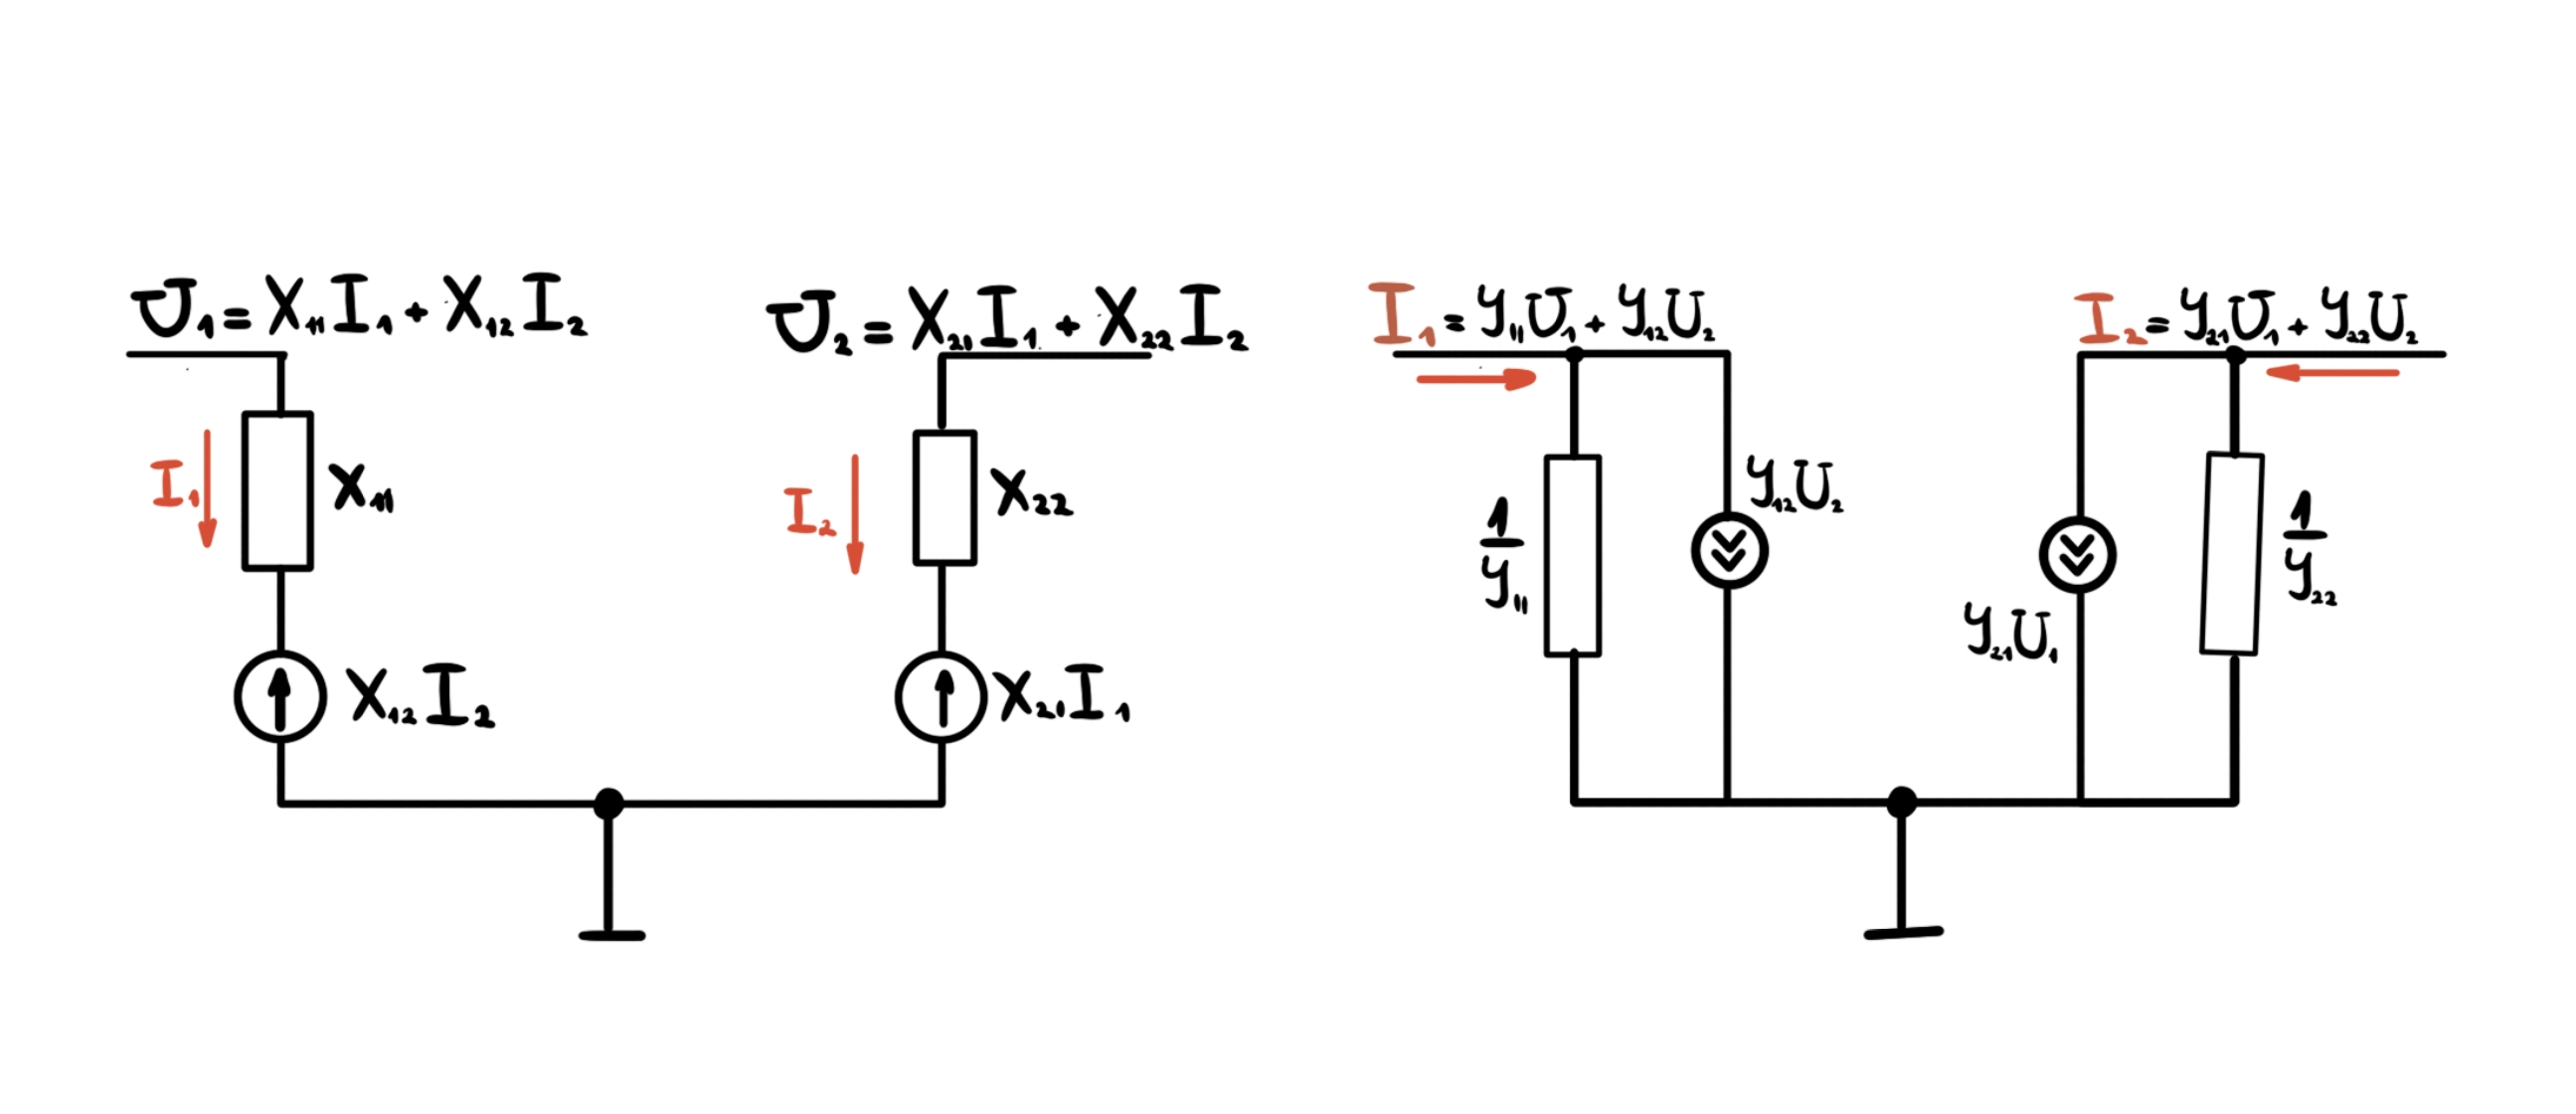
\includegraphics[width=1\textwidth]{Images/X_and_Y.jpg}
    \caption{Эквивалентные схемы с X- и Y-параметрами}
    \label{fig:X_and_Y}
\end{figure}
Заметим, что если матрица X-параметров является невырожденной, то соответствующая этому трехполюснику матрица Y-параметров 
является обратной к матрице X-параметров.

$$
\begin{pmatrix}
Y_{11} & Y_{12} \\ Y_{21} & Y_{22}\\
\end{pmatrix}
=
\begin{pmatrix}
X_{11} & X_{12} \\ X_{21} & X_{22}\\
\end{pmatrix}^{-1}
$$
Нас же сейчас будет интересовать частный случай, при котором матрица параметров является симметричной, то 
есть: $X_{21} = X_{12}; Y_{21} = Y_{12}$. В таком случае эквивалентные схемы трехполюсников задаются более 
простыми моделями: для X-параметров это схема из трех сопротивлений под названием \textbf{звезда}. А для Y-параметров - 
схема из трех проводимостей под названием \textbf{трегуольник}.
\begin{figure}[h!]
    \centering
    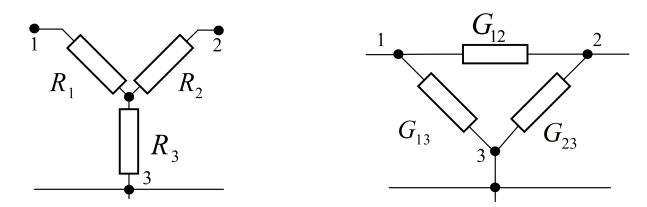
\includegraphics[width=0.8\textwidth]{Images/Star_triangle.png}
    \caption{Схемы ``звезда'' и ``треугольник''}
    \label{fig:star_delta}
\end{figure}
В задании вашей лабораторной работы просят проверить формулу для X-параметров. Давайте найдем ее.
$$
\begin{cases}
U_1 = X_{11}I_1 + X_{12}I_2 \\
U_2 = X_{21}I_1 + X_{22}I_2 \\
\end{cases}
$$
Действуем примерно также, как при вычислении Т-образной схемы. Избавляемся от тока $I_2$ осавляя выходной порт на 
холостом ходу. На входной порт подаем ток $I_0$
$$
\begin{cases}
U_1 = X_{11}I_0 \\
U_2 = X_{21}I_0 \\
\end{cases}
$$
В нашей схеме ток $I_0$ течет через резисторы $R_1$ и $R_3$ находим связь с входным напряжением: $U_1 = (R_1 + R_3)I_0$. 
Через резистор $R_2$ ток не течет, поэтому $U_2 = R_3I_0$.
Отсюда находим: $X_{11} = R_1 + R_3; \quad X_{21} = R_3$.
\textbf{Точно также} (автору уже реально лень) для нахождения второй пары, на холостой ход ставится уже входной порт, а на 
выходной подается ток $I_0$ и Симметрично получается: $X_{12} = R_3; \quad X_{22} = R_2 + R_3$.
Получившаяся матрица X-параметров:
$$
\begin{pmatrix} U_1\\ U_2\\\end{pmatrix}
=
\begin{pmatrix}
R_1 + R_3 & R_3 \\ R_3 & R_2 + R_3\\
\end{pmatrix}
\begin{pmatrix} I_1\\ I_2\\\end{pmatrix}
$$
Действуя аналогичным образом можно найти матрицу Y-параметров для треугольника.
$$
\begin{pmatrix} I_1\\ I_2\\\end{pmatrix}
=
\begin{pmatrix}
G_{12}+G_{13} & -G_{12} \\ -G_{12} & G_{12} + G_{23}\\
\end{pmatrix}
\begin{pmatrix} U_1\\ U_2\\\end{pmatrix}
$$
\subsection*{Техника перехода звезда-треугольник}
Предположим, что для некоторого трехполюсника была получена симметричная матрица X-параметров. Это значит, что мы можем заменить 
исходный трехполюсник звездой. Однако если матрица является невырожденной, значит этот же трехполюсник можно описать и с помощью 
Y-параметров, найдя симметричную матрицу Y-параметров, как обратную к симметричной матрице X-параметров.
Но трехполюсник описываемый симметричной матрицей Y-параметров можно заменить эквивалентным треугольником. Теперь если убрать из 
рассуждения промежуточный трехполюсник, то окажется, что мы нашли способ перейди от звезды к треугольнику:
$$
X^{-1} = Y \quad \Leftrightarrow \quad
\begin{pmatrix}
R_1 + R_3 & R_3 \\ R_3 & R_2 + R_3\\
\end{pmatrix}^{-1}
=
\begin{pmatrix}
G_{13} + G_{12} & -G_{12} \\ -G_{12} & G_{23}+G_{12}\\
\end{pmatrix}
$$
Вспомним, что обратная матрица к матрице 2x2 считается довольно просто.
Для матрицы $A = \begin{pmatrix} a & b \\ c & d \end{pmatrix}$ обратная матрица $A^{-1}$ находится как: 
$$A^{-1} = \frac{1}{\det(A)} \begin{pmatrix} d & -b \\ -c & a \end{pmatrix}$$
где $\det(A)$ — это определитель матрицы $A$, который равен: $\det(A) = ad - bc$.
Займемся вычислением обратной матрицы X-параметров.
$$
\det X = (R_1 + R_3)(R_2+R_3) - R_3^2 = R_1R_2 + R_2R_3+R_1R_3
$$
$$
X^{-1} = \frac{1}{R_1R_2 + R_2R_3+R_1R_3}
\begin{pmatrix}
R_2 + R_3 & -R_3 \\ -R_3 & R_1 + R_3\\
\end{pmatrix}^{-1}
=
\begin{pmatrix}
G_{13} + G_{12} & -G_{12} \\ -G_{12} & G_{23}+G_{12}\\
\end{pmatrix}
$$
Заметим в дух матрицах соответствеие элементов: $R_1 \rightarrow G_{23};\; R_2 \rightarrow 
G_{13};\; R_3 \rightarrow G_{12}$.
Таким образом получаем:
$$
\begin{array}{l}
\frac{R_1}{R_1R_2 + R_2R_3+R_1R_3} = G_{23} \\
\frac{R_2}{R_1R_2 + R_2R_3+R_1R_3} = G_{13} \\
\frac{R_3}{R_1R_2 + R_2R_3+R_1R_3} = G_{12} \\
\end{array}
$$
Вспомним,что проводимости и сопротивления связаня по формуле $R = \frac{1}{G}$.
$$
\begin{array}{l}
\frac{1}{G_{23}} = R_{23} = R_2 + \frac{R_2R_3}{R_1} + R_3 \\
\frac{1}{G_{13}} = R_{13} = R_1 + R_3 + \frac{R_1R_3}{R_2} \\
\frac{1}{G_{23}} = R_{23} = \frac{R_1R_2}{R_3} + R_2 + R_1 \\
\end{array}
$$
Формулы пересчета трегольника в звезду получаются нахождением матрицы X-параметров, через обратную 
матрицу Y-параметров.

\end{document}